%\VignetteIndexEntry{1) Tutorial on using variancePartition}
%\VignettePackage{variancePartition}
%\VignetteEngine{knitr::knitr}
%\VignetteEncoding{UTF-8}


% To compile this document
% cd /Users/gabrielhoffman/workspace/repos
% R 
% library('knitr'); rm(list=ls()); knit('variancePartition/vignettes/variancePartition.Rnw')
% knitr::knit('variancePartition.Rnw')

\documentclass[12pt]{article}\usepackage[]{graphicx}\usepackage[]{xcolor}
% maxwidth is the original width if it is less than linewidth
% otherwise use linewidth (to make sure the graphics do not exceed the margin)
\makeatletter
\def\maxwidth{ %
  \ifdim\Gin@nat@width>\linewidth
    \linewidth
  \else
    \Gin@nat@width
  \fi
}
\makeatother

\definecolor{fgcolor}{rgb}{0.251, 0.251, 0.251}
\newcommand{\hlnum}[1]{\textcolor[rgb]{0.816,0.125,0.439}{#1}}%
\newcommand{\hlstr}[1]{\textcolor[rgb]{0.251,0.627,0.251}{#1}}%
\newcommand{\hlcom}[1]{\textcolor[rgb]{0.502,0.502,0.502}{\textit{#1}}}%
\newcommand{\hlopt}[1]{\textcolor[rgb]{0,0,0}{#1}}%
\newcommand{\hlstd}[1]{\textcolor[rgb]{0.251,0.251,0.251}{#1}}%
\newcommand{\hlkwa}[1]{\textcolor[rgb]{0.125,0.125,0.941}{#1}}%
\newcommand{\hlkwb}[1]{\textcolor[rgb]{0,0,0}{#1}}%
\newcommand{\hlkwc}[1]{\textcolor[rgb]{0.251,0.251,0.251}{#1}}%
\newcommand{\hlkwd}[1]{\textcolor[rgb]{0.878,0.439,0.125}{#1}}%
\let\hlipl\hlkwb

\newenvironment{knitrout}{}{} % an empty environment to be redefined in TeX
\usepackage{alltt}

\newcommand{\lowtilde}{\raise.17ex\hbox{$\scriptstyle\mathtt{\sim}$}}



\RequirePackage[]{/Users/gabrielhoffman/prog/R-4.3.0/library/BiocStyle/resources/tex/Bioconductor}
\AtBeginDocument{\bibliographystyle{/Users/gabrielhoffman/prog/R-4.3.0/library/BiocStyle/resources/tex/unsrturl}}


\usepackage[position=top]{subfig}
\usepackage{blkarray}

\bioctitle[Vignette for variancePartition]{ \Biocpkg{variancePartition}:\\Quantifying and interpreting drivers\\of variation in multilevel gene\\expression experiments}

\author{Gabriel Hoffman\\ 
\small{Pamela Sklar Division of Psychiatric Genomics} \\
\small{Icahn Institute for Genomics and Multiscale Biology}\\
\small{Department of Genetics and Genomic Sciences}\\
\small{Icahn School of Medicine at Mount Sinai}}
\IfFileExists{upquote.sty}{\usepackage{upquote}}{}
\begin{document}

\maketitle

\begin{abstract}
  \noindent
  Gene expression datasets are complicated and have multiple sources of biological and technical variation.  These datasets have recently become more complex as it is now feasible to assay gene expression from the same individual in multiple tissues or at multiple time points.  The \Rpackage{variancePartition} package implements a statistical method to quantify the contribution of multiple sources of variation and decouple within/between-individual variation.  In addition, \Rpackage{variancePartition} produces results at the gene-level to identity genes that follow or deviate from the genome-wide trend.

  \vspace{2cm}
  \noindent
  \textbf{variancePartition version:} 1.31.16
\end{abstract}
  


\newpage

\tableofcontents

\pagebreak
\section{Overview}

The \Rpackage{variancePartition} package provides a general framework for understanding drivers of variation in gene expression in experiments with complex designs.  A typical application would consider a dataset of gene expression from individuals sampled in multiple tissues or multiple time points where the goal is to understand variation within versus between individuals and tissues.  \Rpackage{variancePartition} use a linear mixed model to partition the variance attributable to multiple variables in the data.  The analysis is built on top of the \Rpackage{lme4} package \cite{Bates2015}, and some basic knowledge about linear mixed models will give you some intuition about the behavior of \Rpackage{variancePartition} \cite{Pinheiro2000, Galecki2010}


\subsection{Inputs}

There are three components to an analysis: 
\begin{itemize}
 \item[1)] {\bf Gene expression data:}
 	In general, this is a matrix of normalized gene expression values with genes as rows and experiments as columns. \\

 	\begin{itemize}[align=left]
 		\item[-- Count-based quantification:] \Rcode{featureCounts} \cite{Liao2014}, \Rcode{HTSeq} \cite{Anders2015}\\ 
 			Counts mapping to each gene can be normalized using counts per million (CPM), reads per kilobase per million (RPKM) or fragments per kilobase per million (FPKM).  These count results can be processed with \Rpackage{limma}/\Rcode{voom} \cite{Law2014} to model the precision of each observation or \Rpackage{DESeq2} \cite{Love2014}.\\

 		\item[-- Isoform quantification:] \Rcode{kallisto} \cite{Bray2015}, \Rcode{sailfish} \cite{Patro2014}, \Rcode{salmon} \cite{Patro2015}, \Rcode{RSEM} \cite{Li2011f}, \Rcode{cufflinks} \cite{Trapnell2010}\\
 				These perform isoform-level quantification using reads that map to multiple transcripts.  Quantification values can be read directly into \R{}, or processed with \Rpackage{ballgown} \cite{Frazee2015} or \Rpackage{tximport} \cite{Soneson2015}.\\
 		
 		\item[-- Microarray data:] any standard normalization such as \Rcode{rma} in the \Rpackage{oligo} \cite{oligoBioc} package can be used.    \\   
 	\end{itemize}

 \item[2)] {\bf Meta-data about each experiment:}  A \Rcode{data.frame} with information about each experiment such as patient ID, tissue, sex, disease state, time point, batch, etc.\\ 

 \item[2)] {\bf Formula indicating which meta-data variables to consider:} An R{} formula such as\\ 
 \Rcode{$\sim$ Age + (1|Individual) + (1|Tissue) + (1|Batch) }
 indicating which meta-data variables should be used in the analysis.
\end{itemize}


 \Rpackage{variancePartition} will assess the contribution of each meta-data variable to variation in gene expression and can report the intra-class correlation for each variable.   


\pagebreak
\section{Running an analysis}

A typical analysis with \Rpackage{variancePartition} is only a few lines of \R{} code, assuming the expression data has already been normalized.  Normalization is a separate topic, and I address it briefly 
in Section \ref{sec:normalize_RNA_Seq}.

The simulated dataset included as an example contains measurements of 200 genes from 100 samples.  These samples include assays from 3 tissues across 25 individuals processed in 4 batches.  The individuals range in age from 36 to 73.  A typical \Rpackage{variancePartition} analysis will assess the contribution of each aspect of the study design (i.e. individual, tissue, batch, age) to the expression variation of each gene.  The analysis will prioritize these axes of variation based on a genome-wide summary and give results at the gene-level to identity genes that follow or deviate from this genome-wide trend.   The results can be visualized using custom plots and can be used for downstream analysis.

\subsection{Standard application}


\begin{knitrout}
\definecolor{shadecolor}{rgb}{0.941, 0.941, 0.941}\color{fgcolor}\begin{kframe}
\begin{alltt}
\hlcom{# load library}
\hlkwd{library}\hlstd{(}\hlstr{"variancePartition"}\hlstd{)}

\hlcom{# load simulated data:}
\hlcom{# geneExpr: matrix of gene expression values}
\hlcom{# info: information/metadata about each sample}
\hlkwd{data}\hlstd{(varPartData)}

\hlstd{form} \hlkwb{<-} \hlopt{~} \hlstd{Age} \hlopt{+} \hlstd{(}\hlnum{1} \hlopt{|} \hlstd{Individual)} \hlopt{+} \hlstd{(}\hlnum{1} \hlopt{|} \hlstd{Tissue)} \hlopt{+} \hlstd{(}\hlnum{1} \hlopt{|} \hlstd{Batch)}

\hlstd{varPart} \hlkwb{<-} \hlkwd{fitExtractVarPartModel}\hlstd{(geneExpr, form, info)}

\hlcom{# vp <- sortCols( varPart )}

\hlcom{# plotPercentBars( vp[1:10,] )}

\hlcom{# plotVarPart( vp )}
\end{alltt}
\end{kframe}
\end{knitrout}

\begin{knitrout}
\definecolor{shadecolor}{rgb}{0.941, 0.941, 0.941}\color{fgcolor}\begin{kframe}
\begin{alltt}
\hlcom{# load library}
\hlkwd{library}\hlstd{(}\hlstr{"variancePartition"}\hlstd{)}

\hlcom{# load simulated data:}
\hlcom{# geneExpr: matrix of gene expression values}
\hlcom{# info: information/metadata about each sample}
\hlkwd{data}\hlstd{(varPartData)}

\hlcom{# Specify variables to consider}
\hlcom{# Age is continuous so model it as a fixed effect}
\hlcom{# Individual and Tissue are both categorical,}
\hlcom{# so model them as random effects}
\hlcom{# Note the syntax used to specify random effects}
\hlstd{form} \hlkwb{<-} \hlopt{~} \hlstd{Age} \hlopt{+} \hlstd{(}\hlnum{1} \hlopt{|} \hlstd{Individual)} \hlopt{+} \hlstd{(}\hlnum{1} \hlopt{|} \hlstd{Tissue)} \hlopt{+} \hlstd{(}\hlnum{1} \hlopt{|} \hlstd{Batch)}

\hlcom{# Fit model and extract results}
\hlcom{# 1) fit linear mixed model on gene expression}
\hlcom{# If categorical variables are specified,}
\hlcom{#     a linear mixed model is used}
\hlcom{# If all variables are modeled as fixed effects,}
\hlcom{# 		a linear model is used}
\hlcom{# each entry in results is a regression model fit on a single gene}
\hlcom{# 2) extract variance fractions from each model fit}
\hlcom{# for each gene, returns fraction of variation attributable}
\hlcom{# 		to each variable}
\hlcom{# Interpretation: the variance explained by each variables}
\hlcom{# after correcting for all other variables}
\hlcom{# Note that geneExpr can either be a matrix,}
\hlcom{# and EList output by voom() in the limma package,}
\hlcom{# or an ExpressionSet}
\hlstd{varPart} \hlkwb{<-} \hlkwd{fitExtractVarPartModel}\hlstd{(geneExpr, form, info)}

\hlcom{# sort variables (i.e. columns) by median fraction}
\hlcom{# 		of variance explained}
\hlstd{vp} \hlkwb{<-} \hlkwd{sortCols}\hlstd{(varPart)}

\hlcom{# Figure 1a}
\hlcom{# Bar plot of variance fractions for the first 10 genes}
\hlkwd{plotPercentBars}\hlstd{(vp[}\hlnum{1}\hlopt{:}\hlnum{10}\hlstd{, ])}
\hlcom{#}
\hlcom{# Figure 1b}
\hlcom{# violin plot of contribution of each variable to total variance}
\hlkwd{plotVarPart}\hlstd{(vp)}
\end{alltt}
\end{kframe}
\end{knitrout}

\Rpackage{variancePartition} includes a number of custom plots to visualize the results.  Since \Rpackage{variancePartition} attributes the fraction of total variation attributable to each aspect of the study design, these fractions naturally sum to 1.  \Rcode{plotPercentBars} plots the partitioning results for a subset of genes (Figure 1a), and \Rcode{plotVarPart} shows a genome-wide violin plot of the distribution of variance explained by each variable across all genes (Figure 1b).  (Note that these plots show results in terms of \underline{percentage} of variance explained, while the results are stored in terms of the \underline{fraction}.)
  
\begin{figure}[hb]
\centering
\subfloat[]{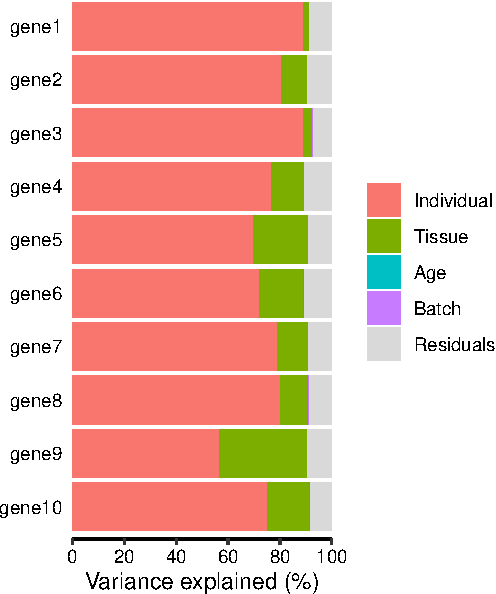
\includegraphics[width=.45\textwidth]{figure/simResult-1}}\quad
\subfloat[]{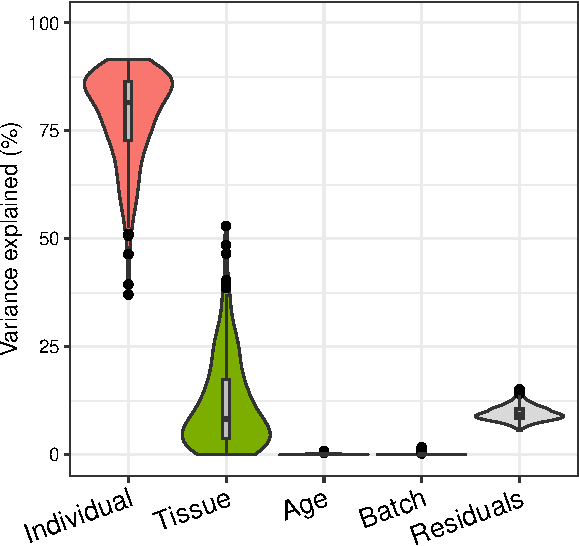
\includegraphics[width=.45\textwidth]{figure/simResult-2}}
\caption{
 \Rpackage{variancePartition} example on simulated data}
\label{fig:lab}
\end{figure}

The core functions of \Rpackage{variancePartition} work seemlessly with gene expression data stored as a \Robject{matrix}, \Robject{data.frame}, \Robject{EList} from \Rpackage{limma} or \Robject{ExpressionSet} from \Rpackage{Biobase}.  \Rcode{fitExtractVarPartModel()} returns an object that stores the variance fractions for each gene and each variable in the formula specified.  These fractions can be accessed just like a \Rcode{data.frame}:

\begin{knitrout}
\definecolor{shadecolor}{rgb}{0.941, 0.941, 0.941}\color{fgcolor}\begin{kframe}
\begin{alltt}
\hlcom{# Access first entries}
\hlkwd{head}\hlstd{(varPart)}
\end{alltt}
\begin{verbatim}
##          Batch Individual Tissue      Age Residuals
## gene1 0.000158      0.890 0.0247 4.53e-05    0.0847
## gene2 0.000000      0.806 0.1010 3.34e-04    0.0926
## gene3 0.002422      0.890 0.0356 1.47e-03    0.0704
## gene4 0.000000      0.769 0.1253 1.01e-03    0.1048
## gene5 0.000000      0.700 0.2091 3.87e-05    0.0911
## gene6 0.002344      0.722 0.1679 2.72e-03    0.1048
\end{verbatim}
\begin{alltt}
\hlcom{# Access first entries for Individual}
\hlkwd{head}\hlstd{(varPart}\hlopt{$}\hlstd{Individual)}
\end{alltt}
\begin{verbatim}
## [1] 0.890 0.806 0.890 0.769 0.700 0.722
\end{verbatim}
\begin{alltt}
\hlcom{# sort genes based on variance explained by Individual}
\hlkwd{head}\hlstd{(varPart[}\hlkwd{order}\hlstd{(varPart}\hlopt{$}\hlstd{Individual,} \hlkwc{decreasing} \hlstd{=} \hlnum{TRUE}\hlstd{), ])}
\end{alltt}
\begin{verbatim}
##           Batch Individual  Tissue      Age Residuals
## gene43  0.00000      0.914 0.01174 3.78e-04    0.0735
## gene174 0.00000      0.911 0.00973 2.02e-03    0.0770
## gene111 0.00000      0.907 0.00839 9.74e-04    0.0839
## gene127 0.00000      0.904 0.01384 5.08e-04    0.0821
## gene151 0.00608      0.903 0.00000 1.35e-05    0.0910
## gene91  0.00000      0.900 0.01414 1.11e-06    0.0856
\end{verbatim}
\end{kframe}
\end{knitrout}

\subsubsection{Saving plot to file}

In order to save the plot to a file, use the \Rcode{ggsave} function:
\begin{knitrout}
\definecolor{shadecolor}{rgb}{0.941, 0.941, 0.941}\color{fgcolor}\begin{kframe}
\begin{alltt}
\hlstd{fig} \hlkwb{<-} \hlkwd{plotVarPart}\hlstd{(vp)}
\hlkwd{ggsave}\hlstd{(file, fig)}
\end{alltt}
\end{kframe}
\end{knitrout}

\pagebreak
\subsection{Plot expression stratified by other variables}

\Rpackage{variancePartition} also includes plotting functions to visualize the variation across a variable of interest. \Rcode{plotStratify} plots the expression of a gene stratified by the specified variable.  In the example dataset, users can plot a gene expression trait stratified by Tissue (Figure 2a) or Individual (Figure 2b).

\begin{knitrout}
\definecolor{shadecolor}{rgb}{0.941, 0.941, 0.941}\color{fgcolor}\begin{kframe}
\begin{alltt}
\hlcom{# get gene with the highest variation across Tissues}
\hlcom{# create data.frame with expression of gene i and Tissue}
\hlcom{# 		type for each sample}
\hlstd{i} \hlkwb{<-} \hlkwd{which.max}\hlstd{(varPart}\hlopt{$}\hlstd{Tissue)}
\hlstd{GE} \hlkwb{<-} \hlkwd{data.frame}\hlstd{(}\hlkwc{Expression} \hlstd{= geneExpr[i, ],} \hlkwc{Tissue} \hlstd{= info}\hlopt{$}\hlstd{Tissue)}

\hlcom{# Figure 2a}
\hlcom{# plot expression stratified by Tissue}
\hlkwd{plotStratify}\hlstd{(Expression} \hlopt{~} \hlstd{Tissue, GE,} \hlkwc{main} \hlstd{=} \hlkwd{rownames}\hlstd{(geneExpr)[i])}
\hlcom{#}
\hlcom{# get gene with the highest variation across Individuals}
\hlcom{# create data.frame with expression of gene i and Tissue}
\hlcom{# 		type for each sample}
\hlstd{i} \hlkwb{<-} \hlkwd{which.max}\hlstd{(varPart}\hlopt{$}\hlstd{Individual)}
\hlstd{GE} \hlkwb{<-} \hlkwd{data.frame}\hlstd{(}
  \hlkwc{Expression} \hlstd{= geneExpr[i, ],}
  \hlkwc{Individual} \hlstd{= info}\hlopt{$}\hlstd{Individual}
\hlstd{)}

\hlcom{# Figure 2b}
\hlcom{# plot expression stratified by Tissue}
\hlstd{label} \hlkwb{<-} \hlkwd{paste}\hlstd{(}\hlstr{"Individual:"}\hlstd{,} \hlkwd{format}\hlstd{(varPart}\hlopt{$}\hlstd{Individual[i]} \hlopt{*} \hlnum{100}\hlstd{,}
  \hlkwc{digits} \hlstd{=} \hlnum{3}
\hlstd{),} \hlstr{"%"}\hlstd{)}
\hlstd{main} \hlkwb{<-} \hlkwd{rownames}\hlstd{(geneExpr)[i]}
\hlkwd{plotStratify}\hlstd{(Expression} \hlopt{~} \hlstd{Individual, GE,}
  \hlkwc{colorBy} \hlstd{=} \hlkwa{NULL}\hlstd{,}
  \hlkwc{text} \hlstd{= label,} \hlkwc{main} \hlstd{= main}
\hlstd{)}
\end{alltt}
\end{kframe}
\end{knitrout}

\begin{figure}[h]
\centering
\subfloat[Tissue]{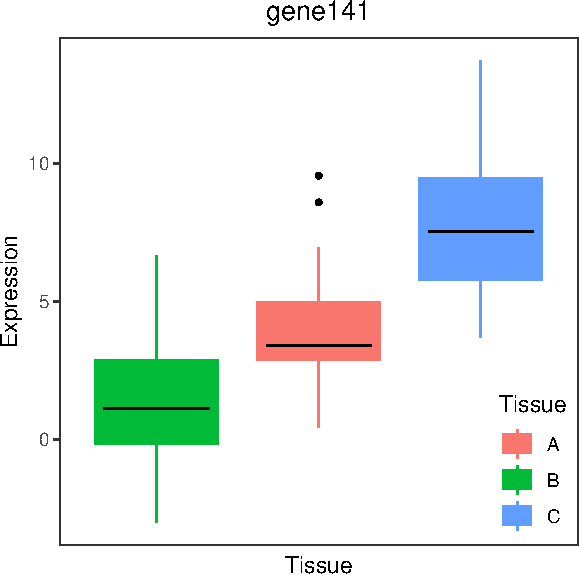
\includegraphics[width=.45\textwidth]{figure/plotStratify-1}}\quad
\subfloat[Individual]{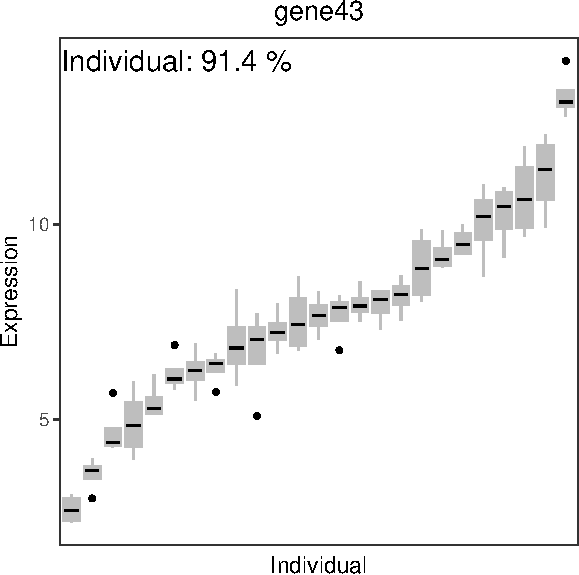
\includegraphics[width=.45\textwidth]{figure/plotStratify-2}}
\caption{ Plot gene expression stratified by {\bf a)} Tissue and {\bf b)} Individual}
\label{fig:Stratify}
\end{figure}

For gene141, variation across tissues explains 52.9\% of variance in gene expression.
For gene43, variation across Individuals explains 91.4\% of variance in gene expression.  


\subsection{Intuition about the backend}

At the heart of \Rcode{variancePartition}, a regression model is fit for each gene separately and summary statistics are extracted and reported to the user for visualization and downstream analysis.  For a single model fit, \Rcode{calcVarPart} computes the fraction of variance explained by each variable.  \Rcode{calcVarPart} is defined by this package, and computes these statistics from either a fixed effects model fit with \Rcode{lm} or a linear mixed model fit with \Rcode{lmer}.  \Rcode{fitExtractVarPart} loops over each gene, fits the regression model and returns the variance fractions reported by \Rcode{calcVarPart}.

Fitting the regression model and extracting variance statistics can also be done directly:
\begin{knitrout}
\definecolor{shadecolor}{rgb}{0.941, 0.941, 0.941}\color{fgcolor}\begin{kframe}
\begin{alltt}
\hlkwd{library}\hlstd{(}\hlstr{"lme4"}\hlstd{)}

\hlcom{# fit regression model for the first gene}
\hlstd{form_test} \hlkwb{<-} \hlstd{geneExpr[}\hlnum{1}\hlstd{, ]} \hlopt{~} \hlstd{Age} \hlopt{+} \hlstd{(}\hlnum{1} \hlopt{|} \hlstd{Individual)} \hlopt{+} \hlstd{(}\hlnum{1} \hlopt{|} \hlstd{Tissue)}
\hlstd{fit} \hlkwb{<-} \hlkwd{lmer}\hlstd{(form_test, info,} \hlkwc{REML} \hlstd{=} \hlnum{FALSE}\hlstd{)}

\hlcom{# extract variance statistics}
\hlkwd{calcVarPart}\hlstd{(fit)}
\end{alltt}
\begin{verbatim}
## Individual     Tissue        Age  Residuals 
##   8.90e-01   2.47e-02   4.35e-05   8.50e-02
\end{verbatim}
\end{kframe}
\end{knitrout}

\pagebreak
\section{Interpretation}

\Rpackage{variancePartition} fits a linear (mixed) model that jointly considers the contribution of all specified variables on the expression of each gene.  It uses a multiple regression model so that the effect of each variable is assessed while jointly accounting for all others\footnote{\href{https://www.r-bloggers.com/2011/03/anova-–-type-iiiiii-ss-explained/}{Standard ANOVA} implemented in R involves refitting the model while dropping terms, but is aimed at hypothesis testing.  \Rpackage{variancePartition}'s \Rcode{calcVarPart} is aimed at estimating variance fractions.  It uses a single fit of the linear (mixed) model and evaluates the sum of squares of each term and the sum of squares of the total model fit.}. However, we note that like any multiple regression model, high correlation bewtween fixed or random effect variables (see Section \ref{sec:canCor}) can produce unstable estimates and it can be challanging to identify which variable is responsible for the expression variation.

The results of \Rpackage{variancePartition} give insight into the expression data at multiple levels.  Moreover, a single statistic often has multiple equivalent interpretations while only one is relevant to the biological question.  Analysis of the example data in Figure 1 gives some strong interpretations. 

Considering the median across all genes,
\begin{itemize}
\item[1)] variation across individuals explains a median of 81.5\% of the variation in expression, after correcting for tissue, batch and age
\item[2)] variation across tissues explains a median of 8.2\% of the variation in expression, after correcting for other the variables
\item[3)] variation across batches is negligible after correcting for variation due to other variables
\item[4)] the effect of age is negligible after correcting for other variables 
\item[5)] correcting for individual, tissue, batch and age leaves a median of 9.3\% of the total variance in expression.
\end{itemize} 

These statistics also have a natural interpretation in terms of the intra-class correlation (ICC), the correlation between observations made from samples in the same group.  

Considering the median across across all genes and all experiments,
\begin{itemize}
\item[1)] the ICC for \underline{individual} is 81.5\%.
\item[2)] the ICC for \underline{tissue} is 8.2\%.
\item[3)] two randomly selected gene measurements from same \underline{individual}, but regardless of \underline{tissue}, \underline{batch} or \underline{age}, have a correlation of 81.5\%. 
\item[4)] two randomly selected gene measurements from same \underline{tissue}, but regardless of \underline{individual}, \underline{batch} or \underline{age}, have a correlation of 8.2\%.
\item[5)] two randomly selected gene measurements from the same \underline{individual} {\it and} same \underline{tissue}, but regardless of \underline{batch} and \underline{age}, have an correlation of 81.5\% + 8.2\% = 89.7\%.
\end{itemize} 

Note that that the ICC here is interpreted as the ICC after correcting for all other variables in the model.

These conclusions are based on the genome-wide median across all genes, but the same type of statements can be made at the gene-level.  Moreover, care must be taken in the interpretation of nested variables.  For example, \Rcode{Age} is nested within \Rcode{Individual} since the multiple samples from each individual are taken at the same age.  Thus the effect of \Rcode{Age} removes some variation from being explained by \Rcode{Individual}.  This often arises when considering variation across individuals and across sexes: any cross-sex variation is a component of the cross-individual variation.  So the total variation across individuals is the sum of the fraction of variance explained by \Rcode{Sex} and \Rcode{Individual}.  This nesting/summing of effects is common for variables that are properties of the individual rather than the sample.  For example, sex and ethnicity are always properties of the individual.  Variables like age and disease state can be properties of the individual, but could also vary in time-course or longitudinal  experiments.  The the interpretation depends on the experimental design.

The real power of \Rpackage{variancePartition} is to identify specific genes that follow or deviate from the genome-wide trend.  The gene-level statistics can be used to identify a subset of genes that are enriched for specific biological functions.  For example, we can ask if the 500 genes with the highest variation in expression across tissues (i.e. the long tail for tissue in Figure 1a) are enriched for genes known to have high tissue-specificity.

% {\it Note:} The percent variance explained is equivalent to the ICC only when the formula takes the simple form $$ \sim (1|A) + (1|B) + C + ...$$  

%For complex formulas using varying coefficient models $$\sim (1|A/B)+...$$ or correlated random intercepts $$\sim (A|B) + ...$$ the percent variance explained is a useful statistical, but does not correspond to ICC. 



\subsection{Should a variable be modeled as fixed or random effect?}
 
Categorical variables should (almost) always be modeled as a random effect.  The difference between modeling a categorical variable as a fixed versus random effect is minimal when the sample size is large compared to the number of categories (i.e. levels).  So variables like disease status, sex or time point will not be sensitive to modeling as a fixed versus random effect.  However, variables with many categories like \Rcode{Individual} {\it must} be modeled as a random effect in order to obtain statistically valid results.  So to be on the safe side, categorical variable should be modeled as a random effect.  

% \R{} and \Rpackage{variancePartition} handle catagorical variables stored as a \Rcode{factor} very naturally.  If categorical variables are stored as an \Rcode{integer} or \Rcode{character}, they must be converted to a \Rcode{factor} before being used with \Rpackage{variancePartition}

\Rpackage{variancePartition} fits two types of models: 
\begin{itemize}
	\item[1)] linear mixed model where \underline{all} categorical variables are modeled as random effects and all continuous variables are fixed effects.  The function \Rcode{lmer} from \Rpackage{lme4} is used to fit this model.

	\item[2)] fixed effected model, where all variables are modeled as fixed effects. The function \Rcode{lm} is used to fit this model.

\end{itemize}

\subsection{Which variables should be included?}

In my experience, it is useful to include all variables in the first analysis and then drop variables that have minimal effect.  However, like all multiple regression methods, \Rpackage{variancePartition} will divide the contribution over multiple variables that are strongly correlated.  So, for example, including both sex and height in the model will show sex having a smaller contribution to variation gene expression than if height were omitted, since there variables are strongly correlated.  This is a simple example, but should give some intuition about a common issue that arises in analyses with \Rpackage{variancePartition}.

\Rpackage{variancePartition} can naturally assess the contribution of both individual and sex in a dataset.  As expected, genes for which sex explains a large fraction of variation are located on chrX and chrY.  If the goal is to interpret the impact of sex, then there is no issue.  But recall the issue with correlated variables and note that individual is correlated with sex, because each individual is only one sex regardless of how many samples are taken from a individual. It follows that including sex in the model reduces the \underline{apparent} contribution of individual to gene expression.  In other words, the ICC for individual will be different if sex is included in the model.

In general, including variables in the model that do not vary within individual will reduce the apparent contribution of individual as estimated by \Rpackage{variancePartition}.  For example, sex and ethnicity never vary between multiple samples from the same individual and will always reduce the apparent contribution of individual.  However, disease state and age may or may not vary depending on the study design.

In biological datasets technical variability (i.e. batch effects) can often reduce the apparent biological signal.  In RNA-seq analysis, it is common for the the impact of this technical variability to be removed before downstream analysis.  Instead of including these batch variable in the \Rpackage{variancePartition} analysis, it is simple to complete the expression residuals with the batch effects removed and then feeds these residuals to \Rpackage{variancePartition}.  This will increase the fraction of variation explained by biological variables since technical variability is reduced.



\subsubsection{Assess correlation between all pairs of variables}
\label{sec:canCor}

Evaluating the correlation between variables in a important part in interpreting variancePartition results.  When comparing two continuous variables, Pearson correlation is widely used.  But variancePartition includes categorical variables in the model as well.  In order to accommodate the correlation between a continuous and a categorical variable, or two categorical variables we used canonical correlation analysis.  

Canonical Correlation Analysis (CCA) is similar to correlation between two vectors, except that CCA can accommodate matricies as well.  For a pair of variables, canCorPairs assesses the degree to which they co-vary and contain the same information.  Variables in the formula can be a continuous variable or a discrete variable expanded to a matrix (which is done in the backend of a regression model).  For a pair of variables, canCorPairs uses CCA to compute the correlation between these variables and returns the pairwise correlation matrix.

Statistically, let rho be the array of correlation values returned by the standard R function cancor to compute CCA.  canCorPairs returns rho / sum(rho) which is the fraction of the maximum possible correlation. Note that CCA returns correlations values between 0 and 1

\begin{knitrout}
\definecolor{shadecolor}{rgb}{0.941, 0.941, 0.941}\color{fgcolor}\begin{kframe}
\begin{alltt}
\hlstd{form} \hlkwb{<-} \hlopt{~} \hlstd{Individual} \hlopt{+} \hlstd{Tissue} \hlopt{+} \hlstd{Batch} \hlopt{+} \hlstd{Age} \hlopt{+} \hlstd{Height}

\hlcom{# Compute Canonical Correlation Analysis (CCA)}
\hlcom{# between all pairs of variables}
\hlcom{# returns absolute correlation value}
\hlstd{C} \hlkwb{<-} \hlkwd{canCorPairs}\hlstd{(form, info)}

\hlcom{# Plot correlation matrix}
\hlkwd{plotCorrMatrix}\hlstd{(C)}
\end{alltt}
\end{kframe}
\end{knitrout}

\begin{figure}[h]
\centering
\caption{Assess correlation between all pairs of variables}
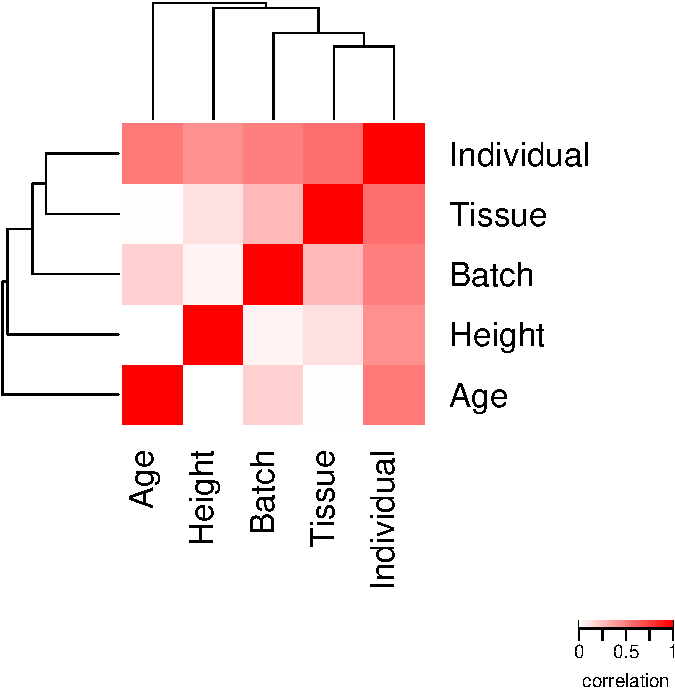
\includegraphics[width=.5\textwidth]{figure/canCorPairs-1}
\label{fig:canCorPairs}
\end{figure}



\pagebreak
\section{Advanced analysis}

\subsection{Extracting additional information from model fits}

Advanced users may want to perform the model fit and extract results in separate steps in order to examine the fit of the model for each gene.  Thus the work of \Rcode{fitExtractVarPart} can be divided into two steps: 1) fit the regression model, and 2) extracting variance statistics. \\    

\begin{knitrout}
\definecolor{shadecolor}{rgb}{0.941, 0.941, 0.941}\color{fgcolor}\begin{kframe}
\begin{alltt}
\hlstd{form} \hlkwb{<-} \hlopt{~} \hlstd{Age} \hlopt{+} \hlstd{(}\hlnum{1} \hlopt{|} \hlstd{Individual)} \hlopt{+} \hlstd{(}\hlnum{1} \hlopt{|} \hlstd{Tissue)} \hlopt{+} \hlstd{(}\hlnum{1} \hlopt{|} \hlstd{Batch)}

\hlcom{# Fit model}
\hlstd{results} \hlkwb{<-} \hlkwd{fitVarPartModel}\hlstd{(geneExpr, form, info)}

\hlcom{# Extract results}
\hlstd{varPart} \hlkwb{<-} \hlkwd{extractVarPart}\hlstd{(results)}
\end{alltt}
\end{kframe}
\end{knitrout}

Note that storing the model fits can use a lot of memory ($\sim$10Gb with 20K genes and 1000 experiments). I do not recommend unless you have a specific need for storing the entire model fit.

Instead, \Rcode{fitVarPartModel} can extract any desired information using any function that accepts the model fit from \Rcode{lm}/\Rcode{lmer}.  The results are stored in a \Rcode{list} and can be used for downstream analysis.

\begin{knitrout}
\definecolor{shadecolor}{rgb}{0.941, 0.941, 0.941}\color{fgcolor}\begin{kframe}
\begin{alltt}
\hlcom{# Fit model and run summary() function on each model fit}
\hlstd{vpSummaries} \hlkwb{<-} \hlkwd{fitVarPartModel}\hlstd{(geneExpr, form, info,} \hlkwc{fxn} \hlstd{= summary)}
\end{alltt}
\end{kframe}
\end{knitrout}

\begin{knitrout}
\definecolor{shadecolor}{rgb}{0.941, 0.941, 0.941}\color{fgcolor}\begin{kframe}
\begin{alltt}
\hlcom{# Show results of summary() for the first gene}
\hlstd{vpSummaries[[}\hlnum{1}\hlstd{]]}
\end{alltt}
\begin{verbatim}
## Linear mixed model fit by maximum likelihood  ['lmerMod']
## Formula: y.local ~ Age + (1 | Individual) + (1 | Tissue) + (1 | Batch)
##    Data: data
## Weights: data$w.local
## Control: control
## 
##      AIC      BIC   logLik deviance df.resid 
##      397      413     -193      385       94 
## 
## Scaled residuals: 
##     Min      1Q  Median      3Q     Max 
## -2.0580 -0.5865  0.0147  0.6603  1.9708 
## 
## Random effects:
##  Groups     Name        Variance Std.Dev.
##  Individual (Intercept) 10.82275 3.2898  
##  Batch      (Intercept)  0.00192 0.0438  
##  Tissue     (Intercept)  0.30010 0.5478  
##  Residual                1.02997 1.0149  
## Number of obs: 100, groups:  Individual, 25; Batch, 4; Tissue, 3
## 
## Fixed effects:
##              Estimate Std. Error t value
## (Intercept) -10.60243    1.09493   -9.68
## Age           0.00318    0.01610    0.20
## 
## Correlation of Fixed Effects:
##     (Intr)
## Age -0.739
\end{verbatim}
\end{kframe}
\end{knitrout}


\subsection{Removing batch effects before fitting model}

Gene expression studies often have substantial batch effects, and \Rpackage{variancePartition} can be used to understand the magnitude of the effects.  However, we often want to focus on biological variables (i.e. individual, tissue, disease, sex) after removing the effect of technical variables.  Depending on the size of the batch effect, I have found it useful to correct for the batch effect first and then perform a \Rpackage{variancePartition} analysis afterward.  Subtracting this batch effect can reduce the total variation in the data, so that the contribution of other variables become clearer.  

Standard analysis:
\begin{knitrout}
\definecolor{shadecolor}{rgb}{0.941, 0.941, 0.941}\color{fgcolor}\begin{kframe}
\begin{alltt}
\hlstd{form} \hlkwb{<-} \hlopt{~} \hlstd{(}\hlnum{1} \hlopt{|} \hlstd{Tissue)} \hlopt{+} \hlstd{(}\hlnum{1} \hlopt{|} \hlstd{Individual)} \hlopt{+} \hlstd{(}\hlnum{1} \hlopt{|} \hlstd{Batch)} \hlopt{+} \hlstd{Age}
\hlstd{varPart} \hlkwb{<-} \hlkwd{fitExtractVarPartModel}\hlstd{(geneExpr, form, info)}
\end{alltt}
\end{kframe}
\end{knitrout}

Analysis on residuals:
\begin{knitrout}
\definecolor{shadecolor}{rgb}{0.941, 0.941, 0.941}\color{fgcolor}\begin{kframe}
\begin{alltt}
\hlkwd{library}\hlstd{(}\hlstr{"limma"}\hlstd{)}
\hlcom{# subtract out effect of Batch}
\hlstd{fit} \hlkwb{<-} \hlkwd{lmFit}\hlstd{(geneExpr,} \hlkwd{model.matrix}\hlstd{(}\hlopt{~}\hlstd{Batch, info))}
\hlstd{res} \hlkwb{<-} \hlkwd{residuals}\hlstd{(fit, geneExpr)}

\hlcom{# fit model on residuals}
\hlstd{form} \hlkwb{<-} \hlopt{~} \hlstd{(}\hlnum{1} \hlopt{|} \hlstd{Tissue)} \hlopt{+} \hlstd{(}\hlnum{1} \hlopt{|} \hlstd{Individual)} \hlopt{+} \hlstd{Age}

\hlstd{varPartResid} \hlkwb{<-} \hlkwd{fitExtractVarPartModel}\hlstd{(res, form, info)}
\end{alltt}
\end{kframe}
\end{knitrout}

Remove batch effect with linear mixed model
\begin{knitrout}
\definecolor{shadecolor}{rgb}{0.941, 0.941, 0.941}\color{fgcolor}\begin{kframe}
\begin{alltt}
\hlcom{# subtract out effect of Batch with linear mixed model}
\hlstd{modelFit} \hlkwb{<-} \hlkwd{fitVarPartModel}\hlstd{(geneExpr,} \hlopt{~} \hlstd{(}\hlnum{1} \hlopt{|} \hlstd{Batch), info)}
\hlstd{res} \hlkwb{<-} \hlkwd{residuals}\hlstd{(modelFit)}

\hlcom{# fit model on residuals}
\hlstd{form} \hlkwb{<-} \hlopt{~} \hlstd{(}\hlnum{1} \hlopt{|} \hlstd{Tissue)} \hlopt{+} \hlstd{(}\hlnum{1} \hlopt{|} \hlstd{Individual)} \hlopt{+} \hlstd{Age}

\hlstd{varPartResid} \hlkwb{<-} \hlkwd{fitExtractVarPartModel}\hlstd{(res, form, info)}
\end{alltt}
\end{kframe}
\end{knitrout}

If the two-step process requires too much memory, the residuals can be computed more efficiently.  Here, run the \Rcode{residuals} function inside the call to \Rcode{fitVarPartModel} to avoid storing the large intermediate results.
\begin{knitrout}
\definecolor{shadecolor}{rgb}{0.941, 0.941, 0.941}\color{fgcolor}\begin{kframe}
\begin{alltt}
\hlcom{# extract residuals directly without storing intermediate results}
\hlstd{residList} \hlkwb{<-} \hlkwd{fitVarPartModel}\hlstd{(geneExpr,} \hlopt{~} \hlstd{(}\hlnum{1} \hlopt{|} \hlstd{Batch), info,}
  \hlkwc{fxn} \hlstd{= residuals}
\hlstd{)}

\hlcom{# convert list to matrix}
\hlstd{residMatrix} \hlkwb{<-} \hlkwd{do.call}\hlstd{(rbind, residList)}
\end{alltt}
\end{kframe}
\end{knitrout}

\subsection{Variation within multiple subsets of the data}
\label{sec:withinSubset}

So far, we have focused on interpreting one variable at a time. But the linear mixed model behind \Rpackage{variancePartition} is a very powerful framework for analyzing variation at multiple levels.  We can easily extend the previous analysis of the contribution of individual and tissue on variation in gene expression to examine the contribution of individual {\it within} each tissue.  This analysis is as easy as specifying a new formula and rerunning  \Rpackage{variancePartition}.  Note that is analysis will only work when there are replicates for at least some individuals within each tissue in order to assess cross-individual variance with in a tissue.

\begin{knitrout}
\definecolor{shadecolor}{rgb}{0.941, 0.941, 0.941}\color{fgcolor}\begin{kframe}
\begin{alltt}
\hlcom{# specify formula to model within/between individual variance}
\hlcom{# separately for each tissue}
\hlcom{# Note that including +0 ensures each tissue is modeled explicitly}
\hlcom{# Otherwise, the first tissue would be used as baseline}
\hlstd{form} \hlkwb{<-} \hlopt{~} \hlstd{(Tissue} \hlopt{+} \hlnum{0} \hlopt{|} \hlstd{Individual)} \hlopt{+} \hlstd{Age} \hlopt{+} \hlstd{(}\hlnum{1} \hlopt{|} \hlstd{Tissue)} \hlopt{+} \hlstd{(}\hlnum{1} \hlopt{|} \hlstd{Batch)}

\hlcom{# fit model and extract variance percents}
\hlstd{varPart} \hlkwb{<-} \hlkwd{fitExtractVarPartModel}\hlstd{(geneExpr, form, info,} \hlkwc{showWarnings} \hlstd{=} \hlnum{FALSE}\hlstd{)}

\hlcom{# violin plot}
\hlkwd{plotVarPart}\hlstd{(}\hlkwd{sortCols}\hlstd{(varPart),} \hlkwc{label.angle} \hlstd{=} \hlnum{60}\hlstd{)}
\end{alltt}
\end{kframe}
\end{knitrout}

\begin{figure}[h]
\centering
\caption{ Variation across individuals within each tissue}
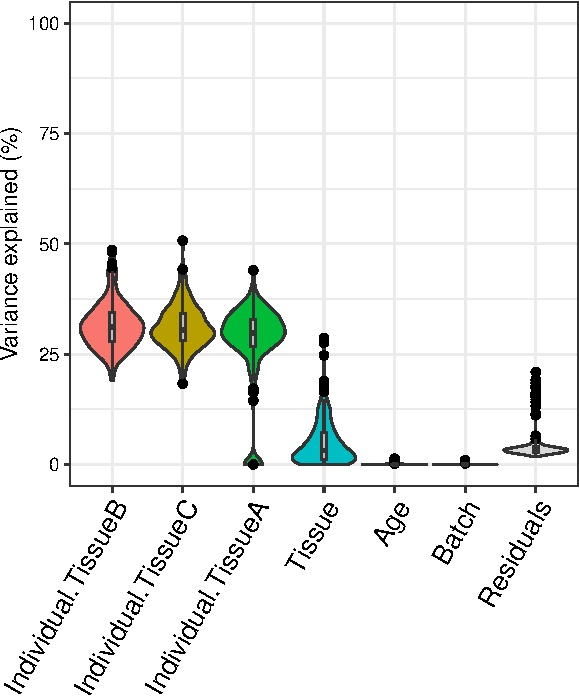
\includegraphics[width=.5\textwidth]{figure/withinTissue-1}
\label{fig:withinTissue}
\end{figure}

This analysis corresponds to a varying coefficient model, where the correlation between individuals varies for each tissue \cite{Pinheiro2000}.  Since the variation across individuals is modeled within each tissue, the total variation explained does not sum to 1 as it does for standard application of \Rpackage{variancePartition}.  So interpretation as intra-class does not strictly apply and use of \Rcode{plotPercentBars} is no longer applicable.  Yet the variables in the study design are still ranked in terms of their genome-wide contribution to expression variation, and results can still be analyzed at the gene level.  See Section \ref{sec:variationWithAcross} for statistical details.


\subsection{Detecting problems caused by collinearity of variables}
\label{sec:collinearity}
Including variables that are highly correlated can produce misleading results and overestimate the contribution of variables modeled as fixed effects.  This is usually not an issue, but can arise when statistically redundant variables are included in the model.   In this case, the model is ``degenerate'' or ``computationally singular'' and parameter estimates from this model are not meaningful.  Dropping one or more of the covariates will fix this problem.\\
\\
A check of collinearity is built into \Rcode{fitVarPartModel} and \Rcode{fitExtractVarPartModel}, so the user will be warned if this is an issue.\\
\\
Alternatively, the user can use the \Rcode{colinearityScore} function to evaluate whether this is an issue for a single model fit:  

\begin{knitrout}
\definecolor{shadecolor}{rgb}{0.941, 0.941, 0.941}\color{fgcolor}\begin{kframe}
\begin{alltt}
\hlstd{form} \hlkwb{<-} \hlopt{~} \hlstd{(}\hlnum{1} \hlopt{|} \hlstd{Individual)} \hlopt{+} \hlstd{(}\hlnum{1} \hlopt{|} \hlstd{Tissue)} \hlopt{+} \hlstd{Age} \hlopt{+} \hlstd{Height}

\hlcom{# fit model}
\hlstd{res} \hlkwb{<-} \hlkwd{fitVarPartModel}\hlstd{(geneExpr[}\hlnum{1}\hlopt{:}\hlnum{4}\hlstd{, ], form, info)}
\end{alltt}
\end{kframe}
\end{knitrout}
\begin{knitrout}
\definecolor{shadecolor}{rgb}{0.941, 0.941, 0.941}\color{fgcolor}\begin{kframe}
\begin{alltt}
\hlcom{# evaluate the collinearity score on the first model fit}
\hlcom{# this reports the correlation matrix between coefficient estimates}
\hlcom{# for fixed effects}
\hlcom{# the collinearity score is the maximum absolute correlation value}
\hlcom{# If the collinearity score > .99 then the variance partition}
\hlcom{# estimates may be problematic}
\hlcom{# In that case, a least one variable should be omitted}
\hlkwd{colinearityScore}\hlstd{(res[[}\hlnum{1}\hlstd{]])}
\end{alltt}
\begin{verbatim}
## [1] 0.777
## attr(,"vcor")
##             (Intercept)     Age  Height
## (Intercept)       1.000 -0.4191 -0.7774
## Age              -0.419  1.0000 -0.0575
## Height           -0.777 -0.0575  1.0000
\end{verbatim}
\end{kframe}
\end{knitrout}

\subsection{Including weights computed separately}

\Rpackage{variancePartition} automatically used precision weights computed by \Rpackage{voom}, but the user can also specify custom weights using the \Rcode{weightsMatrix} argument.

\begin{knitrout}
\definecolor{shadecolor}{rgb}{0.941, 0.941, 0.941}\color{fgcolor}\begin{kframe}
\begin{alltt}
\hlstd{form} \hlkwb{<-} \hlopt{~} \hlstd{(}\hlnum{1} \hlopt{|} \hlstd{Individual)} \hlopt{+} \hlstd{(}\hlnum{1} \hlopt{|} \hlstd{Tissue)} \hlopt{+} \hlstd{Age} \hlopt{+} \hlstd{Height}

\hlcom{# Specify custom weights}
\hlcom{# In this example the weights are simulated from a}
\hlcom{# uniform distribution and are not meaningful.}
\hlstd{weights} \hlkwb{<-} \hlkwd{matrix}\hlstd{(}\hlkwd{runif}\hlstd{(}\hlkwd{length}\hlstd{(geneExpr)),} \hlkwc{nrow} \hlstd{=} \hlkwd{nrow}\hlstd{(geneExpr))}

\hlcom{# Specify custom weights}
\hlstd{res} \hlkwb{<-} \hlkwd{fitExtractVarPartModel}\hlstd{(geneExpr[}\hlnum{1}\hlopt{:}\hlnum{4}\hlstd{, ], form, info,}
  \hlkwc{weightsMatrix} \hlstd{= weights[}\hlnum{1}\hlopt{:}\hlnum{4}\hlstd{, ]}
\hlstd{)}
\end{alltt}
\end{kframe}
\end{knitrout}

In addition, setting the \Rcode{useWeights=FALSE} will suppress usage of the weights in all cases, i.e. when the weights are specified manually or implicitly with the results of \Rcode{voom}.

\subsection{Including interaction terms}

Typical analysis assumes that the effect of each variable on gene expression does not depend on other variables in the model.  Sometimes this assumption is too strict, and we want to model an interaction effect whereby the effect of \Rcode{Batch} depends on \Rcode{Tissue}.  This can be done easly by specifying an interaction term, \Rcode{(1|Batch:Tissue)}.  Since \Rcode{Batch} has 4 categories and \Rcode{Tissue} has 3, this interaction term implicity models a new \Rcode{3*4 = 12} category variable in the analysis.  This new interaction term will absorb some of the variance from the \Rcode{Batch} and \Rcode{Tissue} term, so an interaction model should always include the two constituent variables.    

Here we fit an interaction model, but we observe that interaction between \Rcode{Batch} and \Rcode{Tissue} does not explain much expression variation.

\begin{knitrout}
\definecolor{shadecolor}{rgb}{0.941, 0.941, 0.941}\color{fgcolor}\begin{kframe}
\begin{alltt}
\hlstd{form} \hlkwb{<-} \hlopt{~} \hlstd{(}\hlnum{1} \hlopt{|} \hlstd{Individual)} \hlopt{+} \hlstd{Age} \hlopt{+} \hlstd{Height} \hlopt{+} \hlstd{(}\hlnum{1} \hlopt{|} \hlstd{Tissue)} \hlopt{+} \hlstd{(}\hlnum{1} \hlopt{|} \hlstd{Batch)} \hlopt{+}
  \hlstd{(}\hlnum{1} \hlopt{|} \hlstd{Batch}\hlopt{:}\hlstd{Tissue)}

\hlcom{# fit model}
\hlstd{vpInteraction} \hlkwb{<-} \hlkwd{fitExtractVarPartModel}\hlstd{(geneExpr, form, info)}

\hlkwd{plotVarPart}\hlstd{(}\hlkwd{sortCols}\hlstd{(vpInteraction))}
\end{alltt}
\end{kframe}
\end{knitrout}

\begin{figure}[h]
\centering
\caption{Fit interaction term}
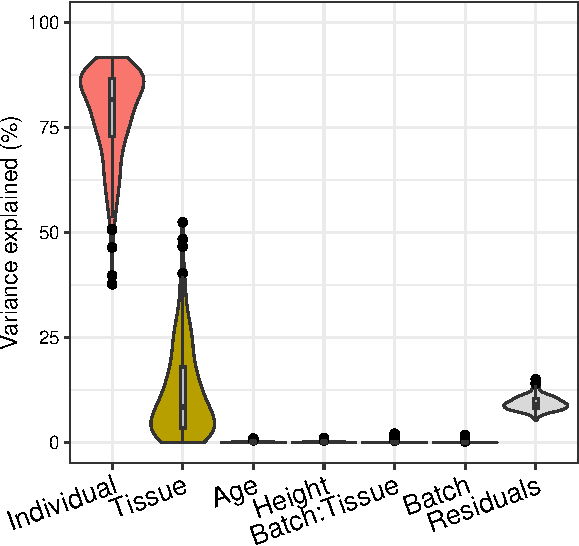
\includegraphics[width=.5\textwidth]{figure/vpInteraction-1}
\label{fig:vpInteraction}
\end{figure}


\pagebreak
\section{Applying \Rpackage{variancePartition} to RNA-seq expression data}
\label{sec:normalize_RNA_Seq}

\Rpackage{variancePartition} works with gene expression data that has already been processed and normalized as for differential expression analysis.

\subsection{Gene-level counts}
\Rcode{featureCounts} \cite{Liao2014} and \Rcode{HTSeq} \cite{Anders2015} report the number of reads mapping to each gene (or exon).  These results are easily read into \R{}.  \Rpackage{limma}/\Rcode{voom} and \Rpackage{DESeq2} are widely used for differential expression analysis of gene- and exon-level counts and can be used to process data before analysis with \Rpackage{variancePartition}.  This section addresses processing and normalization of gene-level counts, but the analysis is the same for exon-level counts.

\subsubsection{\Rpackage{limma}/\Rcode{voom}}
Read RNA-seq counts into \R{}, normalize for library size within and between experiments with TMM \cite{Robinson2010c}, estimate precision weights with \Rpackage{limma}/\Rcode{voom}.

\begin{knitrout}
\definecolor{shadecolor}{rgb}{0.941, 0.941, 0.941}\color{fgcolor}\begin{kframe}
\begin{alltt}
\hlkwd{library}\hlstd{(}\hlstr{"limma"}\hlstd{)}
\hlkwd{library}\hlstd{(}\hlstr{"edgeR"}\hlstd{)}

\hlcom{# identify genes that pass expression cutoff}
\hlstd{isexpr} \hlkwb{<-} \hlkwd{rowSums}\hlstd{(}\hlkwd{cpm}\hlstd{(geneCounts)} \hlopt{>} \hlnum{1}\hlstd{)} \hlopt{>=} \hlnum{0.5} \hlopt{*} \hlkwd{ncol}\hlstd{(geneCounts)}

\hlcom{# create data structure with only expressed genes}
\hlstd{gExpr} \hlkwb{<-} \hlkwd{DGEList}\hlstd{(}\hlkwc{counts} \hlstd{= geneCounts[isexpr, ])}

\hlcom{# Perform TMM normalization}
\hlstd{gExpr} \hlkwb{<-} \hlkwd{calcNormFactors}\hlstd{(gExpr)}

\hlcom{# Specify variables to be included in the voom() estimates of}
\hlcom{# uncertainty.}
\hlcom{# Recommend including variables with a small number of categories}
\hlcom{# that explain a substantial amount of variation}
\hlstd{design} \hlkwb{<-} \hlkwd{model.matrix}\hlstd{(}\hlopt{~}\hlstd{Batch, info)}

\hlcom{# Estimate precision weights for each gene and sample}
\hlcom{# This models uncertainty in expression measurements}
\hlstd{vobjGenes} \hlkwb{<-} \hlkwd{voom}\hlstd{(gExpr, design)}

\hlcom{# Define formula}
\hlstd{form} \hlkwb{<-} \hlopt{~} \hlstd{(}\hlnum{1} \hlopt{|} \hlstd{Individual)} \hlopt{+} \hlstd{(}\hlnum{1} \hlopt{|} \hlstd{Tissue)} \hlopt{+} \hlstd{(}\hlnum{1} \hlopt{|} \hlstd{Batch)} \hlopt{+} \hlstd{Age}

\hlcom{# variancePartition seamlessly deals with the result of voom()}
\hlcom{# by default, it seamlessly models the precision weights}
\hlcom{# This can be turned off with useWeights=FALSE}
\hlstd{varPart} \hlkwb{<-} \hlkwd{fitExtractVarPartModel}\hlstd{(vobjGenes, form, info)}
\end{alltt}
\end{kframe}
\end{knitrout}

\subsubsection{\Rpackage{DESeq2}}

Process and normalize the gene-level counts before running \Rpackage{variancePartition} analysis.
\begin{knitrout}
\definecolor{shadecolor}{rgb}{0.941, 0.941, 0.941}\color{fgcolor}\begin{kframe}
\begin{alltt}
\hlkwd{library}\hlstd{(}\hlstr{"DESeq2"}\hlstd{)}

\hlcom{# create DESeq2 object from gene-level counts and metadata}
\hlstd{dds} \hlkwb{<-} \hlkwd{DESeqDataSetFromMatrix}\hlstd{(}
  \hlkwc{countData} \hlstd{= geneCounts,}
  \hlkwc{colData} \hlstd{= info,}
  \hlkwc{design} \hlstd{=} \hlopt{~}\hlnum{1}
\hlstd{)}

\hlcom{# Estimate library size correction scaling factors}
\hlstd{dds} \hlkwb{<-} \hlkwd{estimateSizeFactors}\hlstd{(dds)}

\hlcom{# identify genes that pass expression cutoff}
\hlstd{isexpr} \hlkwb{<-} \hlkwd{rowSums}\hlstd{(}\hlkwd{fpm}\hlstd{(dds)} \hlopt{>} \hlnum{1}\hlstd{)} \hlopt{>=} \hlnum{0.5} \hlopt{*} \hlkwd{ncol}\hlstd{(dds)}

\hlcom{# compute log2 Fragments Per Million}
\hlcom{# Alternatively, fpkm(), vst() or rlog() could be used}
\hlstd{quantLog} \hlkwb{<-} \hlkwd{log2}\hlstd{(}\hlkwd{fpm}\hlstd{(dds)[isexpr, ]} \hlopt{+} \hlnum{1}\hlstd{)}

\hlcom{# Define formula}
\hlstd{form} \hlkwb{<-} \hlopt{~} \hlstd{(}\hlnum{1} \hlopt{|} \hlstd{Individual)} \hlopt{+} \hlstd{(}\hlnum{1} \hlopt{|} \hlstd{Tissue)} \hlopt{+} \hlstd{(}\hlnum{1} \hlopt{|} \hlstd{Batch)} \hlopt{+} \hlstd{Age}

\hlcom{# Run variancePartition analysis}
\hlstd{varPart} \hlkwb{<-} \hlkwd{fitExtractVarPartModel}\hlstd{(quantLog, form, info)}
\end{alltt}
\end{kframe}
\end{knitrout}

Note that DESeq2 does not compute precision weights like \Rpackage{limma}/\Rcode{voom}, so they are not used in this version of the analysis.

\subsection{Isoform quantification}
	Other software performs isoform-level quantification using reads that map to multiple transcripts.  These include \Rcode{kallisto} \cite{Bray2015}, \Rcode{sailfish} \cite{Patro2014}, \Rcode{salmon} \cite{Patro2015}, \Rcode{RSEM} \cite{Li2011f} and \Rcode{cufflinks} \cite{Trapnell2010}.

\subsubsection{\Rpackage{tximport}}
Quantifications from \Rcode{kallisto}, \Rcode{salmon}, \Rcode{sailfish} and \Rcode{RSEM} can be read into \R{} and processed with the Bioconductor package \Rpackage{tximport}.  The gene- or transcript-level quantifications can be used directly in \Rpackage{variancePartition}.  

\begin{knitrout}
\definecolor{shadecolor}{rgb}{0.941, 0.941, 0.941}\color{fgcolor}\begin{kframe}
\begin{alltt}
\hlkwd{library}\hlstd{(}\hlstr{"tximportData"}\hlstd{)}
\hlkwd{library}\hlstd{(}\hlstr{"tximport"}\hlstd{)}
\hlkwd{library}\hlstd{(}\hlstr{"readr"}\hlstd{)}

\hlcom{# Get data from folder where tximportData is installed}
\hlstd{dir} \hlkwb{<-} \hlkwd{system.file}\hlstd{(}\hlstr{"extdata"}\hlstd{,} \hlkwc{package} \hlstd{=} \hlstr{"tximportData"}\hlstd{)}
\hlstd{samples} \hlkwb{<-} \hlkwd{read.table}\hlstd{(}\hlkwd{file.path}\hlstd{(dir,} \hlstr{"samples.txt"}\hlstd{),} \hlkwc{header} \hlstd{=} \hlnum{TRUE}\hlstd{)}
\hlstd{files} \hlkwb{<-} \hlkwd{file.path}\hlstd{(dir,} \hlstr{"kallisto"}\hlstd{, samples}\hlopt{$}\hlstd{run,} \hlstr{"abundance.tsv"}\hlstd{)}
\hlkwd{names}\hlstd{(files)} \hlkwb{<-} \hlkwd{paste0}\hlstd{(}\hlstr{"sample"}\hlstd{,} \hlnum{1}\hlopt{:}\hlnum{6}\hlstd{)}

\hlstd{tx2gene} \hlkwb{<-} \hlkwd{read.csv}\hlstd{(}\hlkwd{file.path}\hlstd{(dir,} \hlstr{"tx2gene.csv"}\hlstd{))}

\hlcom{# reads results from kallisto}
\hlstd{txi} \hlkwb{<-} \hlkwd{tximport}\hlstd{(files,}
  \hlkwc{type} \hlstd{=} \hlstr{"kallisto"}\hlstd{,} \hlkwc{tx2gene} \hlstd{= tx2gene,}
  \hlkwc{countsFromAbundance} \hlstd{=} \hlstr{"lengthScaledTPM"}
\hlstd{)}

\hlcom{# define metadata (usually read from external source)}
\hlstd{info_tximport} \hlkwb{<-} \hlkwd{data.frame}\hlstd{(}
  \hlkwc{Sample} \hlstd{=} \hlkwd{sprintf}\hlstd{(}\hlstr{"sample%d"}\hlstd{,} \hlnum{1}\hlopt{:}\hlnum{6}\hlstd{),}
  \hlkwc{Disease} \hlstd{=} \hlkwd{c}\hlstd{(}\hlstr{"case"}\hlstd{,} \hlstr{"control"}\hlstd{)[}\hlkwd{c}\hlstd{(}\hlkwd{rep}\hlstd{(}\hlnum{1}\hlstd{,} \hlnum{3}\hlstd{),} \hlkwd{rep}\hlstd{(}\hlnum{2}\hlstd{,} \hlnum{3}\hlstd{))]}
\hlstd{)}

\hlcom{# Extract counts from kallisto}
\hlstd{y} \hlkwb{<-} \hlkwd{DGEList}\hlstd{(txi}\hlopt{$}\hlstd{counts)}

\hlcom{# compute library size normalization}
\hlstd{y} \hlkwb{<-} \hlkwd{calcNormFactors}\hlstd{(y)}

\hlcom{# apply voom to estimate precision weights}
\hlstd{design} \hlkwb{<-} \hlkwd{model.matrix}\hlstd{(}\hlopt{~}\hlstd{Disease,} \hlkwc{data} \hlstd{= info_tximport)}
\hlstd{vobj} \hlkwb{<-} \hlkwd{voom}\hlstd{(y, design)}

\hlcom{# define formula}
\hlstd{form} \hlkwb{<-} \hlopt{~} \hlstd{(}\hlnum{1} \hlopt{|} \hlstd{Disease)}

\hlcom{# Run variancePartition analysis (on only 10 genes)}
\hlstd{varPart_tx} \hlkwb{<-} \hlkwd{fitExtractVarPartModel}\hlstd{(}
  \hlstd{vobj[}\hlnum{1}\hlopt{:}\hlnum{10}\hlstd{, ], form,}
  \hlstd{info_tximport}
\hlstd{)}
\end{alltt}
\end{kframe}
\end{knitrout}

Code to process results from \Rcode{sailfish}, \Rcode{salmon}, \Rcode{RSEM} is very similar.\\
\\
See tutorial at \url{http://bioconductor.org/packages/release/bioc/vignettes/tximport/inst/doc/tximport.html} for more details.



\subsubsection{\Rpackage{ballgown}}

Quantifications from Cufflinks/Tablemaker and RSEM can be processed and read into \R{} with the Bioconductor package \Rpackage{ballgown}.  

\begin{knitrout}
\definecolor{shadecolor}{rgb}{0.941, 0.941, 0.941}\color{fgcolor}\begin{kframe}
\begin{alltt}
\hlkwd{library}\hlstd{(}\hlstr{"ballgown"}\hlstd{)}

\hlcom{# Get data from folder where ballgown is installed}
\hlstd{data_directory} \hlkwb{<-} \hlkwd{system.file}\hlstd{(}\hlstr{"extdata"}\hlstd{,} \hlkwc{package} \hlstd{=} \hlstr{"ballgown"}\hlstd{)}

\hlcom{# Load results of Cufflinks/Tablemaker}
\hlstd{bg} \hlkwb{<-} \hlkwd{ballgown}\hlstd{(}
  \hlkwc{dataDir} \hlstd{= data_directory,} \hlkwc{samplePattern} \hlstd{=} \hlstr{"sample"}\hlstd{,}
  \hlkwc{meas} \hlstd{=} \hlstr{"all"}
\hlstd{)}

\hlcom{# extract gene-level FPKM quantification}
\hlcom{# Expression can be convert to log2-scale if desired}
\hlstd{gene_expression} \hlkwb{<-} \hlkwd{gexpr}\hlstd{(bg)}

\hlcom{# extract transcript-level FPKM quantification}
\hlcom{# Expression can be convert to log2-scale if desired}
\hlstd{transcript_fpkm} \hlkwb{<-} \hlkwd{texpr}\hlstd{(bg,} \hlstr{"FPKM"}\hlstd{)}

\hlcom{# define metadata (usually read from external source)}
\hlstd{info_ballgown} \hlkwb{<-} \hlkwd{data.frame}\hlstd{(}
  \hlkwc{Sample} \hlstd{=} \hlkwd{sprintf}\hlstd{(}\hlstr{"sample%02d"}\hlstd{,} \hlnum{1}\hlopt{:}\hlnum{20}\hlstd{),}
  \hlkwc{Batch} \hlstd{=} \hlkwd{rep}\hlstd{(letters[}\hlnum{1}\hlopt{:}\hlnum{4}\hlstd{],} \hlnum{5}\hlstd{),}
  \hlkwc{Disease} \hlstd{=} \hlkwd{c}\hlstd{(}\hlstr{"case"}\hlstd{,} \hlstr{"control"}\hlstd{)[}\hlkwd{c}\hlstd{(}\hlkwd{rep}\hlstd{(}\hlnum{1}\hlstd{,} \hlnum{10}\hlstd{),} \hlkwd{rep}\hlstd{(}\hlnum{2}\hlstd{,} \hlnum{10}\hlstd{))]}
\hlstd{)}

\hlcom{# define formula}
\hlstd{form} \hlkwb{<-} \hlopt{~} \hlstd{(}\hlnum{1} \hlopt{|} \hlstd{Batch)} \hlopt{+} \hlstd{(}\hlnum{1} \hlopt{|} \hlstd{Disease)}

\hlcom{# Run variancePartition analysis}
\hlcom{# Gene-level analysis}
\hlstd{varPart_gene} \hlkwb{<-} \hlkwd{fitExtractVarPartModel}\hlstd{(}
  \hlstd{gene_expression, form,}
  \hlstd{info_ballgown}
\hlstd{)}

\hlcom{# Transcript-level analysis}
\hlstd{varPart_transcript} \hlkwb{<-} \hlkwd{fitExtractVarPartModel}\hlstd{(}
  \hlstd{transcript_fpkm, form,}
  \hlstd{info_ballgown}
\hlstd{)}
\end{alltt}
\end{kframe}
\end{knitrout}

Note that \Rcode{ballgownrsem} can be used for a similar analysis of \Rcode{RSEM} results.\\
\\
See tutorial at \url{http://bioconductor.org/packages/release/bioc/vignettes/ballgown/inst/doc/ballgown.html} for more details.


\pagebreak
\section{Comparison with other methods on simulated data}

Characterizing drivers of variation in gene expression data has typically relied on principal components analysis (PCA) and hierarchical clustering.  Here I apply these methods to two simulated datasets to demonstrate the additional insight from an analysis with \Rpackage{variancePartition}.  Each simulated dataset comprises 60 experiments from 10 individuals and 3 tissues with 2 biological replicates.  In the first dataset, tissue is the major driver of variation in gene expression(Figure \ref{fig:siteDominant}).  In the second dataset, individual is the major driver of variation in gene expression (Figures \ref{fig:IndivDominant}).

Analysis of simulated data illustrates that PCA identifies the major driver of variation when tissue is dominant and there are only 3 categories.  But the results are less clear when individual is dominant because there are now 10 categories.  Meanwhile, hierarchical clustering identifies the major driver of variation in both cases, but does not give insight into the second leading contributor.

Analysis with \Rpackage{variancePartition} has a number of advantages over these standard methods: 
\begin{itemize}
  \item \Rpackage{variancePartition} provides a natural interpretation of multiple variables
    \begin{itemize}
     \item figures from PCA/hierarchical clustering allow easy interpretation of only one variable
    \end{itemize}
  \vspace{.1in}
  \item \Rpackage{variancePartition} quantifies the contribution of each variable
    \begin{itemize}
      \item PCA/hierarchical clustering give only a visual representation
    \end{itemize}
  \vspace{.1in}
  \item \Rpackage{variancePartition} interprets contribution of each variable to each gene individually for downstream analysis
    \begin{itemize}
     \item PCA/hierarchical clustering produces genome-wide summary and does not allow gene-level interpretation
    \end{itemize} \vspace{2mm}
  \item \Rpackage{variancePartition} can assess contribution of one variable (i.e. Individual) separately in subset of the data defined by another variable (i.e. Tissue)
\end{itemize}









\begin{figure}[h]
\centering
\caption{
  \textbf{Similarity within Tissue is dominant}}
\subfloat[PCA - colored by Tissue]{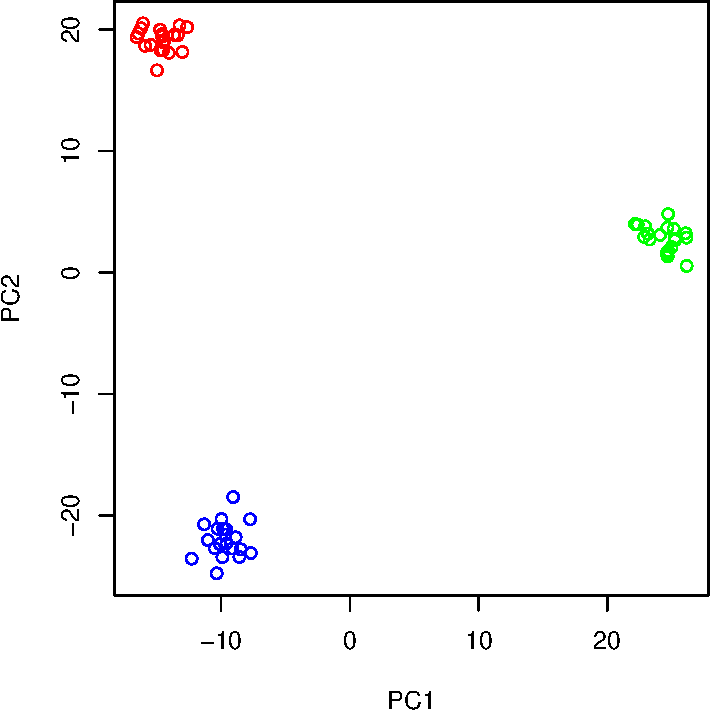
\includegraphics[width=.48\textwidth]{figure/siteDominant-1}}\quad
\subfloat[PCA - colored by Individual]{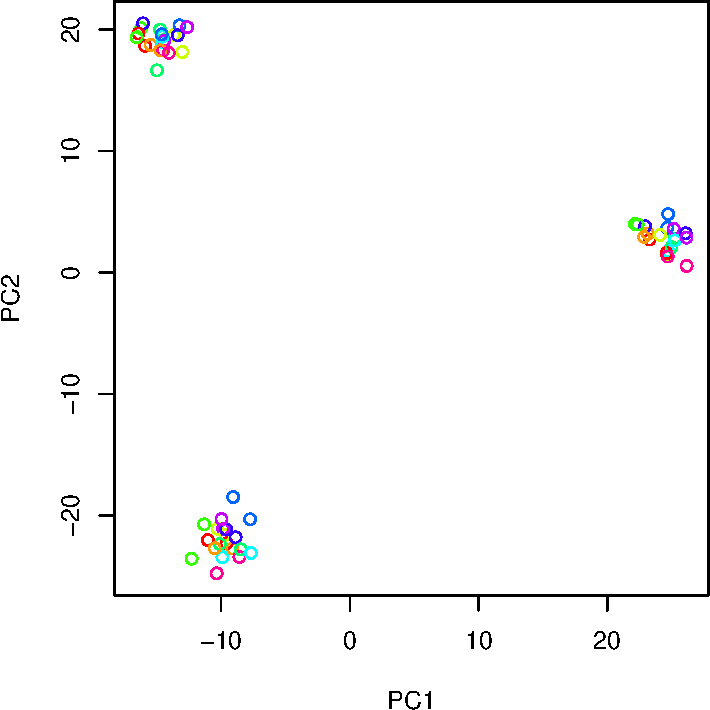
\includegraphics[width=.48\textwidth]{figure/siteDominant-2}}\\
\subfloat[hclust - colored by Tissue]{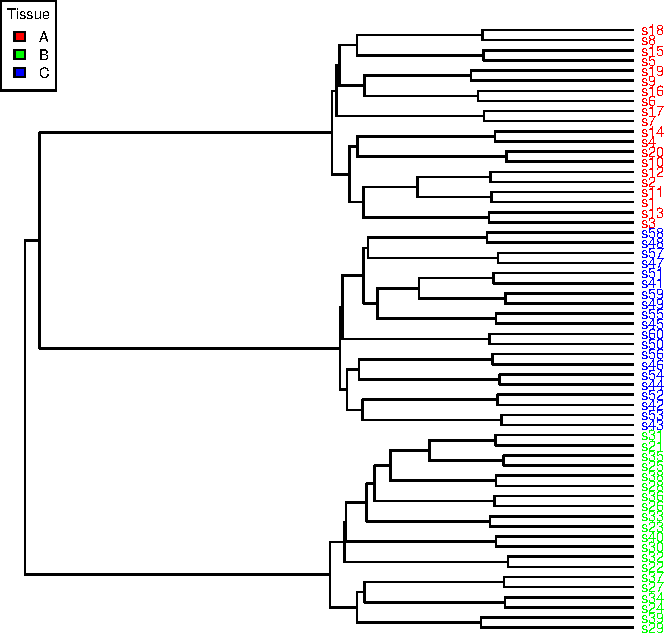
\includegraphics[width=.48\textwidth]{figure/siteDominant-3}}\quad
\subfloat[hclust - colored by Individual]{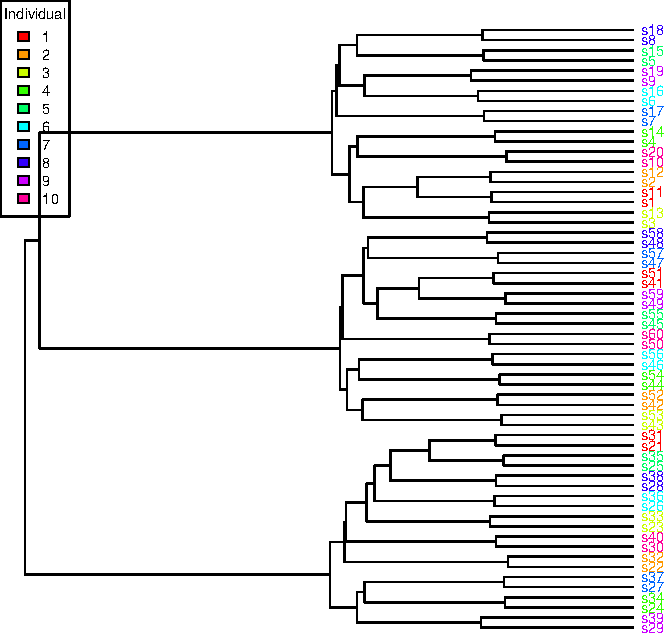
\includegraphics[width=.48\textwidth]{figure/siteDominant-4}}\\
\subfloat[variancePartition]{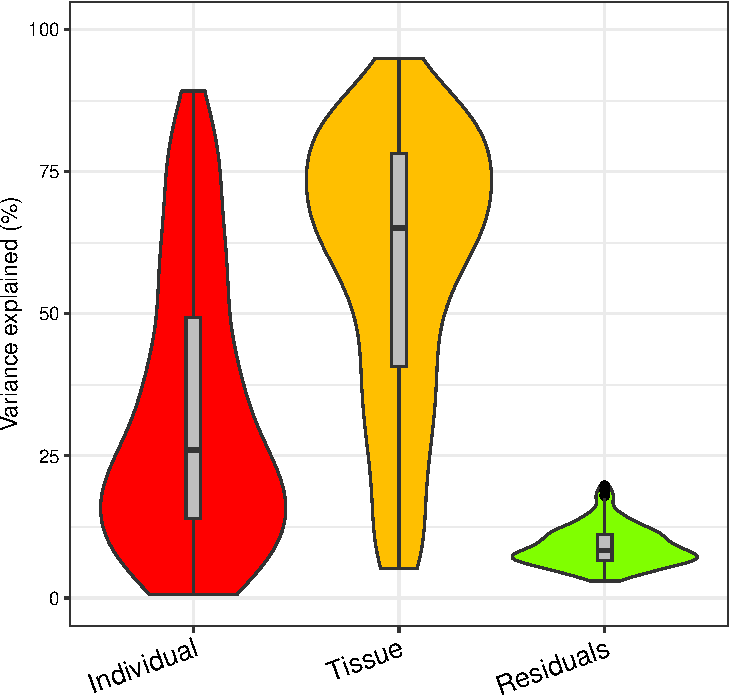
\includegraphics[width=.48\textwidth]{figure/siteDominant-5}}\quad
\subfloat[variancePartition - within Tissue]{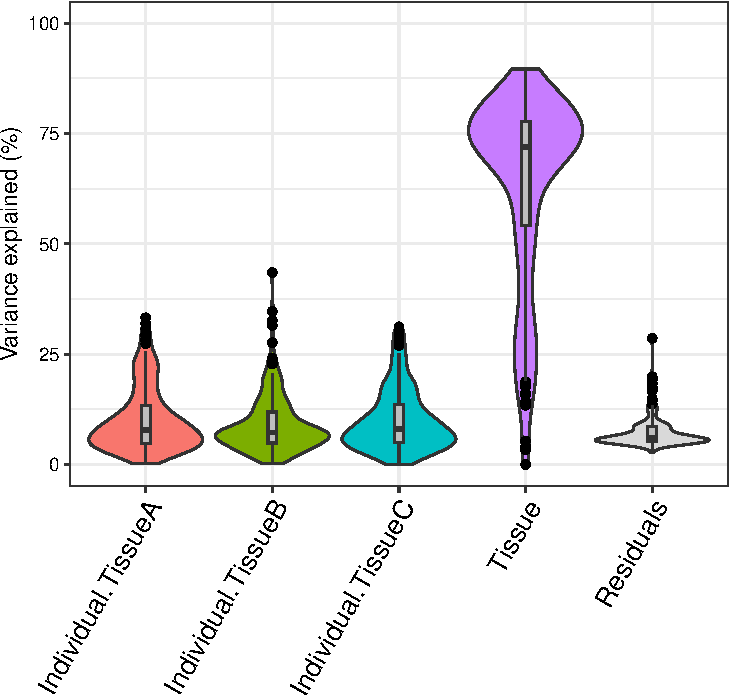
\includegraphics[width=.48\textwidth]{figure/siteDominant-6}}
\label{fig:siteDominant}
\end{figure}

\pagebreak

\begin{figure}[tbp]
\centering
\caption{
  \textbf{Similarity within Individual is dominant}}
\subfloat[PCA - colored by Tissue]{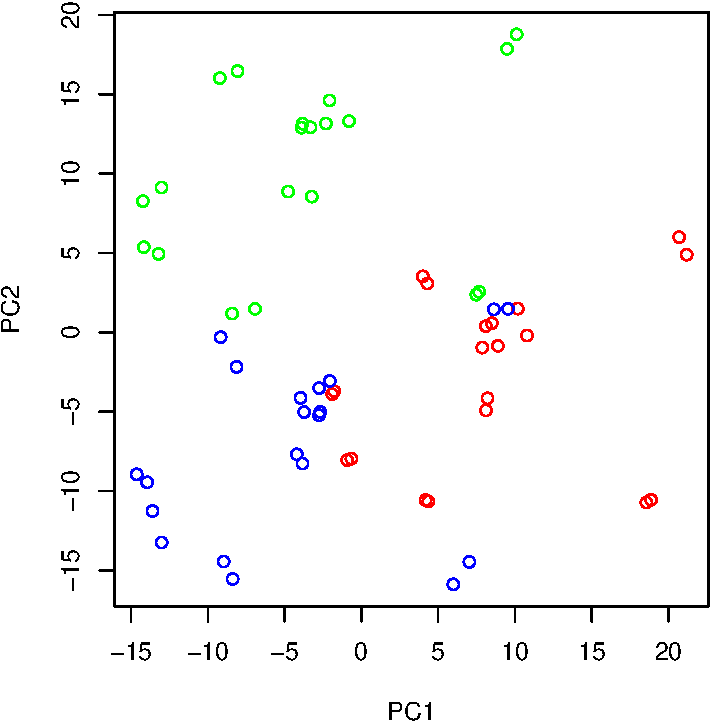
\includegraphics[width=.48\textwidth]{figure/IndivDominant-1}}\quad
\subfloat[PCA - colored by Individual]{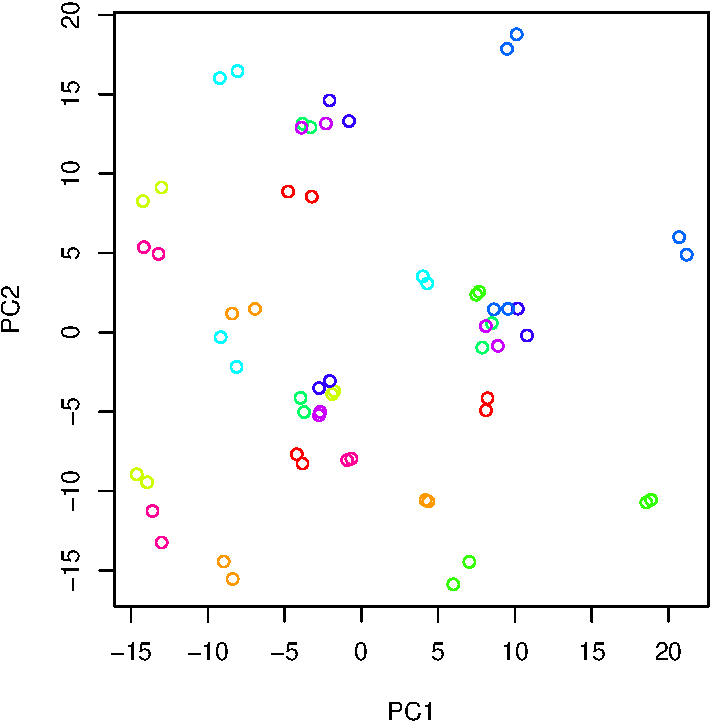
\includegraphics[width=.48\textwidth]{figure/IndivDominant-2}}\\
\subfloat[hclust - colored by Tissue]{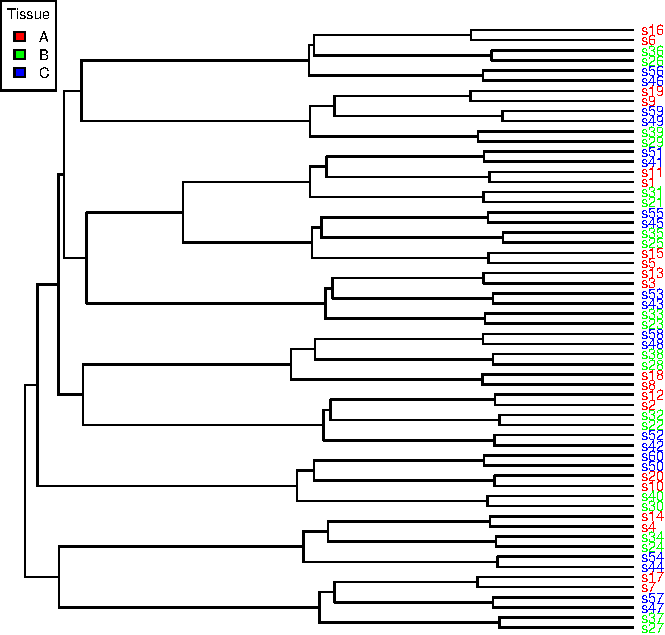
\includegraphics[width=.48\textwidth]{figure/IndivDominant-3}}\quad
\subfloat[hclust - colored by Individual]{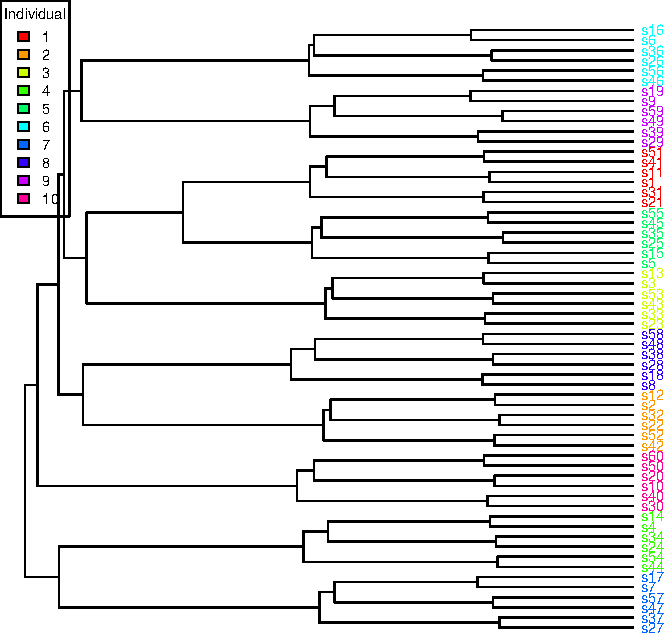
\includegraphics[width=.48\textwidth]{figure/IndivDominant-4}}\\
\subfloat[variancePartition]{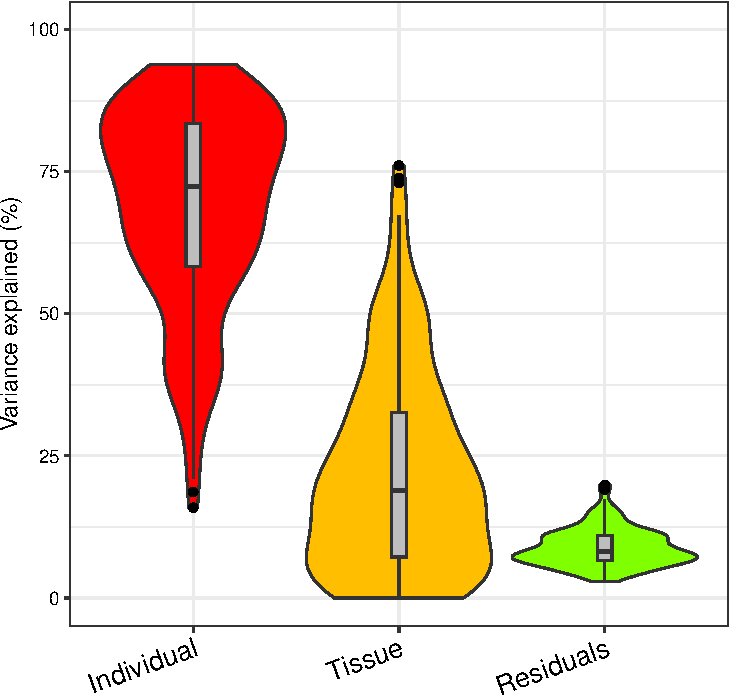
\includegraphics[width=.48\textwidth]{figure/IndivDominant-5}}\quad
\subfloat[variancePartition - within Tissue]{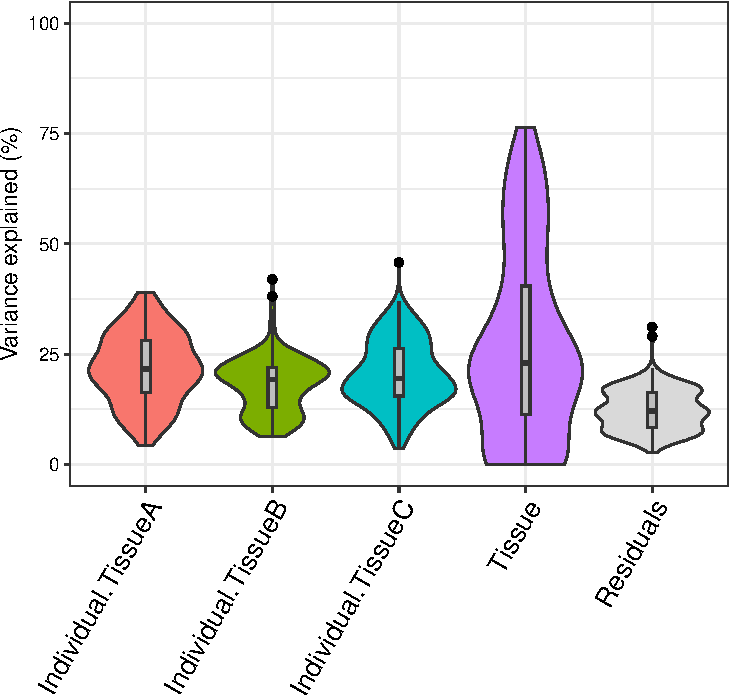
\includegraphics[width=.48\textwidth]{figure/IndivDominant-6}}
\label{fig:IndivDominant}
\end{figure}

\clearpage
\section{Statistical details}

A \Rpackage{variancePartition} analysis evaluates the linear (mixed) model
\begin{eqnarray}
  y &=& \sum_j X_j\beta_j + \sum_k Z_k \alpha_k + \varepsilon \\
  \alpha_k &\sim& \mathcal{N}(0, \sigma^2_{\alpha_k})\\
  \varepsilon &\sim& \mathcal{N}(0, \sigma^2_\varepsilon)
\end{eqnarray}
where $y$ is the expression of a single gene across all samples, $X_j$ is the matrix of $j^{th}$ fixed effect with coefficients $\beta_j$, $Z_k$ is the matrix corresponding to the $k^{th}$ random effect with coefficients $\alpha_k$ drawn from a normal distribution with variance $\sigma^2_{\alpha_k}$.  The noise term, $\varepsilon$, is drawn from a normal distribution with variance $\sigma^2_\varepsilon$.  Parameters are estimated with maximum likelihood, rather than REML, so that fixed effect coefficients, $\beta_j$, are explicitly estimated. \\  
\\
I use the term ``linear (mixed) model'' here since \Rpackage{variancePartition} works seamlessly when a fixed effects model (i.e. linear model) is specified.\\
\\
Variance terms for the fixed effects are computed using the {\it post hoc} calculation  
\begin{eqnarray}
 \hat{\sigma}^2_{\beta_j} = var( X_j \hat{\beta}_j).
\end{eqnarray}
For a fixed effects model, this corresponds to the sum of squares for each component of the model.\\
\\
For a standard application of the linear mixed model, where the effect of each variable is additive, the fraction of variance explained by the $j^{th}$ fixed effect is
\begin{eqnarray}
 \frac{\hat{\sigma}^2_{\beta_j}}{\sum_j \hat{\sigma}^2_{\beta_j} + \sum_k \hat{\sigma}^2_{\alpha_k} + \hat{\sigma}^2_\varepsilon},
\end{eqnarray}
by the $k^{th}$ random effect is 
\begin{eqnarray}
 \frac{\hat{\sigma}^2_{\alpha_k}}{\sum_j \hat{\sigma}^2_{\beta_j} + \sum_k \hat{\sigma}^2_{\alpha_k} + \hat{\sigma}^2_\varepsilon},
 \end{eqnarray}
and the residual variance is 
\begin{eqnarray}
 \frac{\hat{\sigma}^2_{\varepsilon}}{\sum_j \hat{\sigma}^2_{\beta_j} + \sum_k \hat{\sigma}^2_{\alpha_k} + \hat{\sigma}^2_\varepsilon}.
 \end{eqnarray}

\subsection{Implementation in \R{}}

 An \R{} formula is used to define the terms in the fixed and random effects, and \Rcode{fitVarPartModel} fits the specified model for each gene separately.  If random effects are specified, \Rcode{lmer} from \Rpackage{lme4} is used behind the scenes to fit the model, while \Rcode{lm} is used if there are only fixed effects. \Rcode{fitVarPartModel} returns a list of the model fits, and \Rcode{extractVarPart} returns the variance partition statistics for each model in the list.  \Rcode{fitExtractVarPartModel} combines the actions of \Rcode{fitVarPartModel} and \Rcode{extractVarPart} into one function call.  \Rcode{calcVarPart} is called behind the scenes to compute variance fractions for both fixed and mixed effects models, but the user can also call this function directly on a model fit with \Rcode{lm}/\Rcode{lmer}.

\subsection{Interpretation of percent variance explained}
The percent variance explained can be interpreted as the intra-class correlation (ICC) when a special case of Equation 1 is used.  Consider the simplest example of the $i^{th}$ sample from the $k^{th}$ individual 
\begin{eqnarray}
  y_{i,k} = \mu + Z \alpha_{i,k} + e_{i,k}
\end{eqnarray}
with only an intercept term, one random effect corresponding to individual, and an error term.  In this case ICC corresponds to the correlation between two samples from the same individual.  This value is equal to the fraction of variance explained by individual.  For example, consider the correlation between samples from the same individual:
\begin{eqnarray}
  ICC &=& cor( y_{1,k}, y_{2,k}) \\
      &=& cor( \mu + Z \alpha_{1,k}  + e_{1,k}, \mu + Z \alpha_{2,k}  + e_{2,k}) \\
      &=& \frac{cov( \mu + Z \alpha_{1,k}  + e_{1,k}, \mu + Z \alpha_{2,k}  + e_{2,k})}{ \sqrt{ var(\mu + Z \alpha_{1,k} + e_{1,k}) var( \mu + Z \alpha_{2,k} + e_{2,k})}}\\
      &=& \frac{cov(Z \alpha_{1,k}, Z \alpha_{2,k})}{\sigma^2_\alpha + \sigma^2_\varepsilon} \\
      &=& \frac{\sigma^2_\alpha}{\sigma^2_\alpha + \sigma^2_\varepsilon}
\end{eqnarray}
The correlation between samples from different individuals is:
\begin{eqnarray}
  &=& cor( y_{1,1}, y_{1,2}) \\
      &=& cor( \mu + Z \alpha_{1,1} + e_{1,1}, \mu + Z \alpha_{1,2}  + e_{1,2}) \\
      &=& \frac{cov(Z \alpha_{1,1}, Z \alpha_{1,2})}{\sigma^2_\alpha + \sigma^2_\varepsilon} \\
      &=& \frac{0}{\sigma^2_\alpha + \sigma^2_\varepsilon} \\
      &=& 0
\end{eqnarray}
This interpretation in terms of fraction of variation explained (FVE) naturally generalizes to multiple variance components.  Consider two sources of variation, individual and cell type with variances $\sigma^2_{id}$ and $\sigma^2_{cell},$ respectively.  Applying a generalization of the the previous derivation, two samples are correlated according to:

\renewcommand{\arraystretch}{1.8}
\begin{center}
  \begin{tabular}{cccccc}
    \hline
    Individual & cell type & variance & Interpretation & Correlation value\\
    \hline
     same & different &  $\frac{\sigma^2_{id}}{\sigma^2_{id} + \sigma^2_{cell} + \sigma^2_\varepsilon }$ & FVE by individual & $ICC_{individual}$\\%\\[0.1cm] 
    different & same & $\frac{\sigma^2_{cell}}{\sigma^2_{id} + \sigma^2_{cell} + \sigma^2_\varepsilon }$ & FVE by cell type & $ICC_{cell}$\\%\\[0.1cm] 
    same & same & $\frac{\sigma^2_{id} + \sigma^2_{cell}}{\sigma^2_{id} + \sigma^2_{cell} + \sigma^2_\varepsilon }$ & sum of FVE by individual \& cell type & $ICC_{individual,cell}$\\ %\\[0.1cm] \hline
    different & different & $\frac{0}{\sigma^2_{id} + \sigma^2_{cell} + \sigma^2_\varepsilon }$ &  sample are independent  \\%\\[0.1cm] \hline
    \hline
  \end{tabular}
\end{center}

Notice that the correlation between samples from the same individual and same cell type corresponds to the sum of the fraction explained by individual + fraction explained by cell type.  This defines ICC for individual and tissue, as well as the combined ICC and relates these values to FVE.\\
\\
In order to illustrate how this FVE and ICC relate to the correlation between samples in multilevel datasets, consider a simple example of 5 samples from 2 individuals and 2 tissues:

\begin{center}
  \begin{tabular}{|c|c|c|}
    \hline
    Sample & Individual & Cell type \\
    \hline
    a & 1 & T-Cell \\
    b & 1 & T-Cell \\
    c & 1 & monocyte \\
    d & 2 & T-Cell \\
    e & 2 & monocyte\\
    \hline
  \end{tabular}
\end{center} 

Modeling the separate effects of individual and tissue gives the following covariance structure between samples when a linear mixed model is used:
\[
\begin{blockarray}{ccccccc}
&& a & b & c & d & e \\
\begin{block}{cc(ccccc)}
&a &\sigma^2_{id} + \sigma^2_{cell} + \sigma^2_\varepsilon &  & & &\\
&b & \sigma^2_{id} + \sigma^2_{cell} & \sigma^2_{id} + \sigma^2_{cell} + \sigma^2_\varepsilon  & & &\\
cov(y) =  &c & \sigma^2_{id}  & \sigma^2_{id} &\sigma^2_{id} + \sigma^2_{cell} + \sigma^2_\varepsilon  & &\\
&d & \sigma^2_{cell} & \sigma^2_{cell} &0 &\sigma^2_{id} + \sigma^2_{cell} + \sigma^2_\varepsilon  &\\
&e & 0 & 0 &\sigma^2_{cell} & \sigma^2_{id} &\sigma^2_{id} + \sigma^2_{cell} + \sigma^2_\varepsilon \\
\end{block}
\end{blockarray}
 \]
 The covariance matrix is symmetric so that blank entries take the value on the opposite side of the diagonal.  The covariance can be converted to correlation by dividing by $\sigma^2_{id} + \sigma^2_{cell} + \sigma^2_\varepsilon$, and this gives the results from above.  This example generalizes to any number of variance components \cite{Pinheiro2000}.


\subsection{Variation with multiple subsets of the data} \label{sec:variationWithAcross}

The linear mixed model underlying \Rpackage{variancePartition} allows the effect of one variable to depend on the value of another variable.  Statistically, this is called a varying coefficient model \cite{Pinheiro2000, Galecki2010}.  This model arises in  \Rpackage{variancePartition} analysis when the variation explained by individual depends on tissue or cell type.\\
\\
A given sample is only from one cell type, so this analysis asks a question about a subset of the data.  The the data is implicitly divided into subsets base on cell type and variation explained by individual is evaluated within each subset.    The data is not actually divided onto subset, but the statistical model essentially examples samples with each cell type.  This subsetting means that the variance fractions do not sum to 1.\\
\\
Consider a concrete example with variation from across individual and cell types (T-cells and monocytes) with data from the $i^{th}$ sample from the $k^{th}$ individual, sex of $s$ and cell type $c$.  Modeling the variation across individuals within cell type corresponds to 
\begin{eqnarray}
  y_{i,k,s,c} = \mu + Z^{(sex)} \alpha_{i,s} + Z^{(Tcell| id)} \alpha_{i,k,c} + Z^{(monocyte| id)} \alpha_{i,k,c} + e_{i,k,s,c}
\end{eqnarray}    

with corresponding variance components:
\begin{center}
  \begin{tabular}{cc}
    \hline
    Variance component & Interpretation \\
    \hline
    $\sigma^2_{sex}$ & variance across sex (which is the same for all cell types)\\
    $\sigma^2_{(Tcell| id)}$ & variance across individuals within T-cells \\
    $\sigma^2_{(monocyte| id)}$ & variance across individuals within monocytes \\
    $\sigma^2_\varepsilon$ & residual variance \\   
    \hline
  \end{tabular}
\end{center} 

Since the dataset is now divided into multiple subsets, direct interpretation of the fraction of variation explained (FVE) as intra-class correlation does not apply.  Instead, we compute a ``pseudo-FVE" by approximating the total variance attributable to cell type by using a weighted average of the within cell type variances weighted by the sample size within each cell type.  Thus the values of pseudo-FVE do not have the simple interpretation as in the standard application of \Rpackage{variancePartition}, but allows ranking of variables based on genome-wide contribution to variance and analysis of gene-level results.


\subsection{Relationship between \Rpackage{variancePartition} and differential expression}

Differential expression (DE) is widely used to identify gene which show difference is expression between two subsets of the data (i.e. case versus controls). For a single gene, DE analysis measures the difference in mean expression between the two subsets.  (Since expression is usually analyzed on a log scale, DE results are usually shown in terms of log fold changes between the two subsets ).  In Figure \ref{fig:DEVP}, consider two simulated examples of a gene whose expression differs between males and females.  The mean expression in males is 0 and the mean expression in females is 2 in both cases.  Therefore, the fold change is 2 in both cases.\\
\\  
However, the fraction of expression variation explained by sex is very different in these two examples.  In example A, there is very little variation {\it within} each sex, so that variation {\it between} sexes is very high at 91.1\%.  Conversely, example B shows high variation {\it within} sexes, so that variation {\it between} sexes is only 17.8\%.\\
\\
The fact that the fold change or the fraction of variation is significantly different from 0 indicates differential expression between the two sexes.  Yet these two statistics have different interpretations.  The fold change from DE analysis tests a difference in means between two sexes.  The fraction of variation explained compares the variation explained by sex to the total variation.\\
\\
Thus the fraction of variation explained reported by \Rpackage{variancePartition} reflects as different aspect of the data not captured by DE analysis.




\begin{figure}[h]
\centering
\caption{
  \textbf{Compare variancePartition and differential expression}}
\subfloat[Example A]{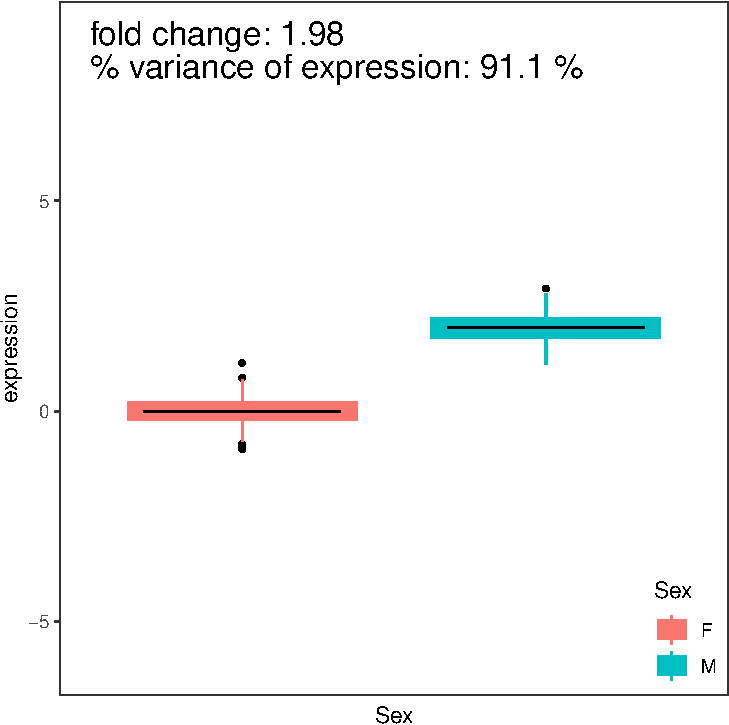
\includegraphics[width=.5\textwidth]{figure/DE-1}}
\subfloat[Example B]{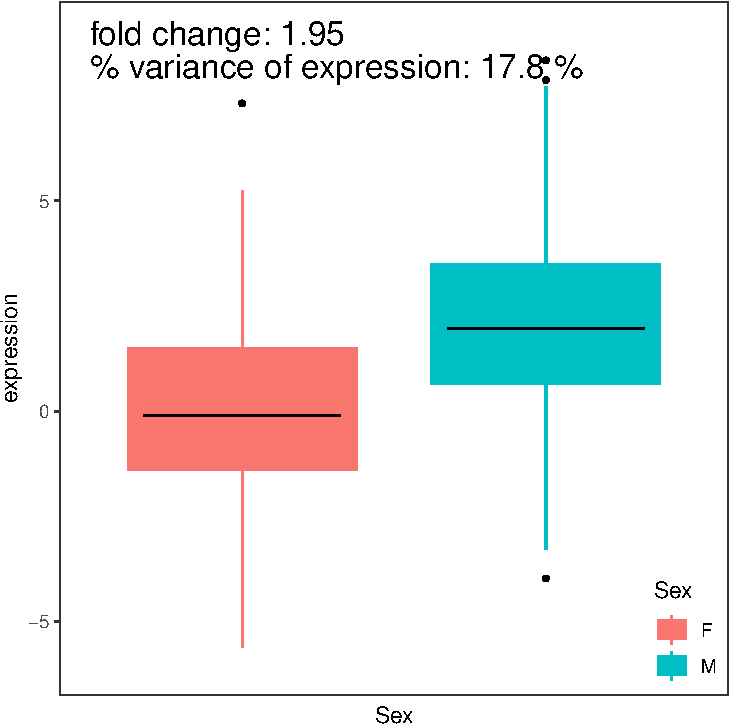
\includegraphics[width=.5\textwidth]{figure/DE-2}}
\label{fig:DEVP}
\end{figure}


\subsection{Modelling error in gene expression measurements}
Uncertainty in the measurement of gene expression can be modeled with precision weights and tests of differentially expression using \Rcode{voom} in \Rpackage{limma} model this uncertainty directly with a heteroskedastic linear regression \cite{Law2014}.  \Rpackage{variancePartition} can use these precision weights in a heteroskedastic linear mixed model implemented in \Rpackage{lme4} \cite{Bates2015}.  These precision weights are used seamlessly by calling \Rcode{fitVarPartModel} or \Rcode{fitExtractVarPartModel} on the output of \Rcode{voom}.  Otherwise the user can specify the weights with the \Rcode{weightsMatrix} parameter.


\pagebreak
\section{Frequently asked questions}

Note that many warnings and errors can be overridden by specifying \newline \Rcode{suppressWarnings=TRUE} for \Rcode{dream()} and \Rcode{showWarnings=FALSE} for \newline\Rcode{fitExtractVarPartModel()} and \Rcode{fitVarPartModel()}.

Interpreting warnings and errors from \Rcode{fitVarPartModel} and \Rcode{fitExtractVarPartModel}:

\subsection{Warnings}

\begin{itemize}
  \item \Rcode{No Intercept term was specified in the formula:\newline The results will not behave as expected and may be very wrong!!}
\end{itemize}
An intercept (i.e. mean term) must be specified order for the results to be statistically valid.  Otherwise, the variance percentages will be {\it very} overestimated.\\

\begin{itemize}
  \item \Rcode{Categorical variables modeled as fixed effect:\newline The results will not behave as expected and may be very wrong!!}
\end{itemize}
If a linear mixed model is used, all categorical variables must be modeled as a random effect.  Alternatively, a fixed effect model can be used by modeling all variables as fixed. \\ 

\begin{itemize}
  \item \Rcode{Cannot have more than one varying coefficient term:\newline The results will not behave as expected and may be very wrong!!}
\end{itemize}
Only one varying coefficient term can be specified.  For example, the formula $\sim$\Rcode{(Tissue+0|Individual) + (Batch+0|Individual)} contains two varying coefficient terms and the results from this analysis are not easily interpretable.  Only a formula with one term like \Rcode{(Tissue+0|Individual)} is allowed. \\ 


\begin{itemize}
  \item \Rcode{executing \%dopar\% sequentially: no parallel backend registered}
\end{itemize}
These functions are optimized to run in parallel using doParallel/doMC.  This warning indicates that a parallelization was not enabled.  This is not a problem, but analysis will take more time.\\

\subsection{Errors}

\begin{itemize}
  \item \Rcode{Colinear score > .99: Covariates in the formula are so strongly\\correlated that the parameter estimates from this model are not\\ meaningful.  Dropping one or more of the covariates will fix this problem}
  \item \Rcode{Error in asMethod(object) : not a positive definite matrix}
  \item \Rcode{In vcov.merMod(fit) : Computed variance-covariance matrix problem:\\not a positive definite matrix; returning NA matrix}
  \item \Rcode{fixed-effect model matrix is rank deficient so dropping 26 columns / coefficients}
\end{itemize}
Including variables that are highly correlated can produce misleading results (see Section \ref{sec:colinearity}).  In this case, parameter estimates from this model are not meaningful.  Dropping one or more of the covariates will fix this problem.\\

\begin{itemize}
  \item \Rcode{Error in checkNlevels(reTrms\$flist, n = n, control) : \newline number of levels of each grouping factor must be < number of observations}
\end{itemize}
This arises when using a varying coefficient model that examines the effect of one variable inside subsets of the data defined by another: $\sim$\Rcode{(A+0|B)}.  See Section \ref{sec:withinSubset}. There must be enough observations of each level of the variable B with each level of variable A.  Consider an example with samples from multiple tissues from a set of individual where we are interested in the variation across individuals within each tissue using the formula: $\sim$ \Rcode{(Tissue+0|Individual)}.  This analysis will only work if there are multiple samples from the same individual in at least one tissue.  If all tissues only have one sample per individual, the analysis will fail and \Rcode{variancePartition} will give this error.\\

\begin{itemize}
  \item \Rcode{Problem with varying coefficient model in formula: should have form (A+0|B)}
\end{itemize}
When analyzing the variation of one variable inside another (Section \ref{sec:withinSubset}), the formula most be specified as \Rcode{(Tissue+0|Individual)}.  This error occurs when the formula contains \Rcode{(Tissue|Individual)} instead.\\

\begin{itemize}
  \item \Rcode{fatal error in wrapper code}
  \item \Rcode{Error in mcfork() : unable to fork, possible reason: Cannot allocate memory}
  \item \Rcode{Error: cannot allocate buffer}
\end{itemize}
 This error occurs when \Rcode{fitVarPartModel} uses too many threads and takes up too much memory.  The easiest solution is to use \Rcode{fitExtractVarPartModel} instead.  Occasionally there is an issue in the parallel backend that is out of my control.  Using fewer threads or restarting \R{} will solve the problem. 

\subsubsection{Errors: Problems removing samples with NA/NaN/Inf values}

\Rpackage{variancePartition} fits a regression model for each gene and drops samples that have NA/NaN/Inf values in each model fit.  This is generally seamless but can cause an issue when a variable specified in the formula no longer varies within the subset of samples that are retained.  Consider an example with variables for sex and age where age is NA for all males samples.  Dropping samples with invalid values for variables included in the formula will retain only female samples.  This will cause \Rpackage{variancePartition} to throw an error because there is now no variation in sex in the retained subset of the data.  This can be resolved by removing either age or sex from the formula.\\
\\
This situtation is indicated by the following errors   
\begin{itemize}
  \item \Rcode{Error: grouping factors must have > 1 sampled level}
  \item \Rcode{Error: Invalid grouping factor specification, Individual}
  \item \Rcode{Error in `contrasts<-`(`*tmp*`, value = contr.funs[1 + isOF[nn]]): \\
  contrasts can be applied only to factors with 2 or more levels}
  \item \Rcode{Error in checkNlevels(reTrms\$flist, n = n, control):\\
  grouping factors must have > 1 sampled level}
\end{itemize}











\section*{Session Info}

\begin{itemize}\raggedright
  \item R version 4.3.0 (2023-04-21), \verb|x86_64-apple-darwin22.4.0|
  \item Locale: \verb|en_US.UTF-8/en_US.UTF-8/en_US.UTF-8/C/en_US.UTF-8/en_US.UTF-8|
  \item Time zone: \verb|America/New_York|
  \item TZcode source: \verb|internal|
  \item Running under: \verb|macOS Ventura 13.5|
  \item Matrix products: default
  \item BLAS:   \verb|/Users/gabrielhoffman/prog/R-4.3.0/lib/libRblas.dylib|
  \item LAPACK: \verb|/usr/local/Cellar/r/4.3.0_1/lib/R/lib/libRlapack.dylib|
; \quad\ LAPACK version3.11.0
  \item Base packages: base, datasets, graphics, grDevices, methods,
    stats, stats4, utils
  \item Other packages: ballgown~2.32.0, Biobase~2.60.0,
    BiocGenerics~0.46.0, BiocParallel~1.34.2, dendextend~1.17.1,
    DESeq2~1.40.1, edgeR~3.42.4, GenomeInfoDb~1.36.1,
    GenomicRanges~1.52.0, ggplot2~3.4.2, IRanges~2.34.1, knitr~1.43,
    limma~3.56.2, lme4~1.1-33, Matrix~1.5-4.1, MatrixGenerics~1.12.0,
    matrixStats~1.0.0, S4Vectors~0.38.1, SummarizedExperiment~1.30.1,
    variancePartition~1.31.16
  \item Loaded via a namespace (and not attached): annotate~1.78.0,
    AnnotationDbi~1.62.1, aod~1.3.2, backports~1.4.1, BiocIO~1.10.0,
    BiocManager~1.30.20, BiocStyle~2.28.0, Biostrings~2.68.1,
    bit~4.0.5, bit64~4.0.5, bitops~1.0-7, blob~1.2.4, boot~1.3-28.1,
    broom~1.0.5, cachem~1.0.8, caTools~1.18.2, cli~3.6.1,
    codetools~0.2-19, colorspace~2.1-0, compiler~4.3.0, corpcor~1.6.10,
    crayon~1.5.2, DBI~1.1.3, DelayedArray~0.26.3, digest~0.6.33,
    dplyr~1.1.2, EnvStats~2.7.0, evaluate~0.21, fANCOVA~0.6-1,
    fansi~1.0.4, farver~2.1.1, fastmap~1.1.1, genefilter~1.82.1,
    generics~0.1.3, GenomeInfoDbData~1.2.10, GenomicAlignments~1.36.0,
    glue~1.6.2, gplots~3.1.3, grid~4.3.0, gridExtra~2.3, gtable~0.3.3,
    gtools~3.9.4, highr~0.10, htmltools~0.5.5, httr~1.4.6,
    iterators~1.0.14, KEGGREST~1.40.0, KernSmooth~2.23-21,
    labeling~0.4.2, lattice~0.21-8, lifecycle~1.0.3, lmerTest~3.1-3,
    locfit~1.5-9.7, magrittr~2.0.3, MASS~7.3-60, memoise~2.0.1,
    mgcv~1.8-42, minqa~1.2.5, munsell~0.5.0, mvtnorm~1.2-2,
    nlme~3.1-162, nloptr~2.0.3, numDeriv~2016.8-1.1, parallel~4.3.0,
    pbkrtest~0.5.2, pillar~1.9.0, pkgconfig~2.0.3, plyr~1.8.8,
    png~0.1-8, purrr~1.0.1, R6~2.5.1, rbibutils~2.2.13,
    RColorBrewer~1.1-3, Rcpp~1.0.11, RCurl~1.98-1.12, Rdpack~2.4,
    remaCor~0.0.17, reshape2~1.4.4, restfulr~0.0.15,
    RhpcBLASctl~0.23-42, rjson~0.2.21, rlang~1.1.1, rmarkdown~2.22,
    Rsamtools~2.16.0, RSQLite~2.3.1, rtracklayer~1.60.0,
    S4Arrays~1.0.4, scales~1.2.1, splines~4.3.0, stringi~1.7.12,
    stringr~1.5.0, survival~3.5-5, sva~3.48.0, tibble~3.2.1,
    tidyr~1.3.0, tidyselect~1.2.0, tools~4.3.0, utf8~1.2.3,
    vctrs~0.6.3, viridis~0.6.3, viridisLite~0.4.2, withr~2.5.0,
    xfun~0.39, XML~3.99-0.14, xtable~1.8-4, XVector~0.40.0, yaml~2.3.7,
    zlibbioc~1.46.0
\end{itemize}





\bibliography{library}

\end{document}
